\chapter*{Editorial}

Looking back over the caving exploration between 2007 and 2012 it almost
seems like it was a pre-ordained story; rags to riches, from a seemingly
hollowed out mountain long past its glory days of exploration to the
longest cave in Slovenia. Living it, it never seemed like this, rather a
more confused and complicated picture, individuals actors without a
script, pulling together in some vague direction but towards perhaps an
achievable objective.

If exploration were a rational expenditure of efforts towards a known
end, the scenes would be rather more simple to describe - we realised
how close we were to the connection of Vrtnarija and Kavkna Jama (M2)
after more carefully analysing the 2007 ``Kill 'em All'' survey data. To
pursue this, we rebolted and rerigged Kavkna Jama in 2008, while
exploring on the other side in Vrtnarija. In 2009 we established a camp
in Vrtnarija at the nearest suitable point to the closest approach, and
used it to massively increase our time at the pushing front. In 2010,
2011 and 2012 we camped deeper in Vrtnarija, while pushing Kavkna Jama
from the surface both during the Summer and on Autumn / Winter trips. In
2012 we connected the systems, forming the longest cave system in
Slovenia, and one in which the vast majority of cave passage is at
depths greater than 500 m.

However, this isn't the real story of exploration. Rather, it is the
story of the people involved that is the true history of Migovec. For
the connection was not made in the obvious location between Kavkna Jama
and Vrtnarija, but down at 650 m of depth, as the result of yet another
successful, to the point of routine, pushing trip. Motivated by the
connection target, during 2008 we flung ourselves into the exploration
of Captain Kangaroo, Vrtnarija. At the grim pushing front were the
youngsters, highly motivated but lacking the experience to go deep.
Lacking in time at the pushing front we determined to go back and camp
in 2009.

``The art of roughing it is in smoothing off the edges.'' Stories of
draughty campsites, cassette players slurring to an undignified
quietness, shivering through the night, and unlabelled plastic bags of
miscellaneous white powder were retold by the experienced members, and
duly obsoleted by careful consideration of the logistics. We went back
with free standing tents, layers of fleece, MP3 players, modern
winter-mix gas stoves and LED fairy lights. We went back to stay, and
almost effortlessly pushed this tough branch of the cave down to 550 m.

This new generation of cavers, who cut their teeth in Captain Kangaroo,
suddenly found themselves with the endurance and know-how to
successfully explore at depth. Though the connection of the systems were
certainly still a major aim of 2010, 2011 and 2012 expeditions, we were
mainly there to push deep new cave passage. We re-established Camp X-Ray
(550 m deep) as our main base, and improved on it year after year till
it became a truly palatial location. And now that the going was once
again deep, we were rejoined by the more experienced members of our
club, for whom the prospect of another grim rift in Captain Kangaroo was
not suitably motivating. And as our collective abilities improved,
normality shifted. Exploring over multi-day camping trips, hot bunking
and the considerable feat of endurance just to reach and return from
these depths became standard practice. That which was just-possible the
year before became the standard trip, that which was beyond our reach
became achievable.

I am proud of the time that I have dedicated towards these expeditions,
and every moment spent with the people involved. There are others in the
club who have contributed very much more. We were all volunteers - we
did all this because we wanted to, but little would get done if we only
did things that were fun. Spending your free-time down caving stores
fettling kit is neither particularly enjoyable nor directly rewarding.
Carries in the hail and rain are arduous and unpleasant. I don't think
it is possible for this document to understate the sacrifice of time and
effort made by expedition members and friends. Forever lacking in
adequate funding and gear, unrecognised and often misunderstood, we have
achieved our exploration on a wing and a prayer.

This exploration report is dedicated to our many friends who assisted,
sponsored, carried, hosted and advised. You all contributed to the
achievements documented herein.

And so, Ninety-Nine years after Apsley Cherry-Garrard returned to South
Kensington with the Penguins Eggs, we return to our college with a minor
news story and a few pretty photos for their website. For those involved
in the exploration of Tolminski Migovec far more precious are the
memories of friendships formed deep within the Hollow Mountain. The
prize was not the destination we arrived at, but the path we forged in
getting here.

We were always in the longest cave in Slovenia, we just hadn't realised.

\attrib{Jarvist Moore Frost}

\begin{verse}
We shall not cease from exploration  \\
And the end of all our exploring  \\
Will be to arrive where we started  \\
And know the place for the first time.  \\
Through the unknown, unremembered gate  \\
When the last of earth left to discover  \\
Is that which was the beginning;  \\
At the source of the longest river  \\
The voice of the hidden waterfall \\
\end{verse}

\attrib{T. S. Eliot}

\chapter{2010}

\section{Vodna Sled}

Vodna Sled 2010 was a clear success - in all we discovered 2.2km of new
passage, all below -500m, all in Vrtnarija using \textsc{Camp
X-Ray} (\textsc{Reloaded}, now a plush four bed camp at -550 m) as a
base. The majority of the discoveries lead from a horizontal series near
\textsc{Zimmer} chamber with numerous un-pushed leads for next year and
over 1.5 km of passage. Significant amounts of exploration also took
place in \textsc{Tolminska Korita} concluding with a connection to the
`deep' level at -653 m, and pushing the \textsc{Republica} streamway
from -744 to -802 m.

\section{Expedition Overview}

Twenty-two expedition members travelled from the UK for a total of 65
person-weeks in the field, with 88 person-trips in our callout roster.
Seventeen from the UK stayed at underground camp, along with six
Slovenes from the local JSPDT club, a total of 95 people-nights at camp.
All successful exploration took place on camping trips. This was the
first expedition for three first-year UK students, all of whom stayed at
underground camp and discovered significant quantities of new cave.

In all, the cave consumed a kilometre of rope for the rerigging of the
main pitch series, and newly explored sections left rigged (or with rope
pulled up) for 2011.

No work during the 2010 expedition went into M2 (Kavkna Jama), directed
towards forging a connection with Vrtnarija. However, during the early
Autumn two JSPDT trips capped through the tight rift at the very end of
the cave (\textasciitilde{}-390m), discovering and then descending a
\textasciitilde{}60m pitch.

The prospects for 2011 are extremely good. The extensive horizontal
development has led to the discovery and initial exploration of a number
of independent streamways and associated pitch series, in a horizontal
slice of the mountain we have never visited.

\begin{figure*}
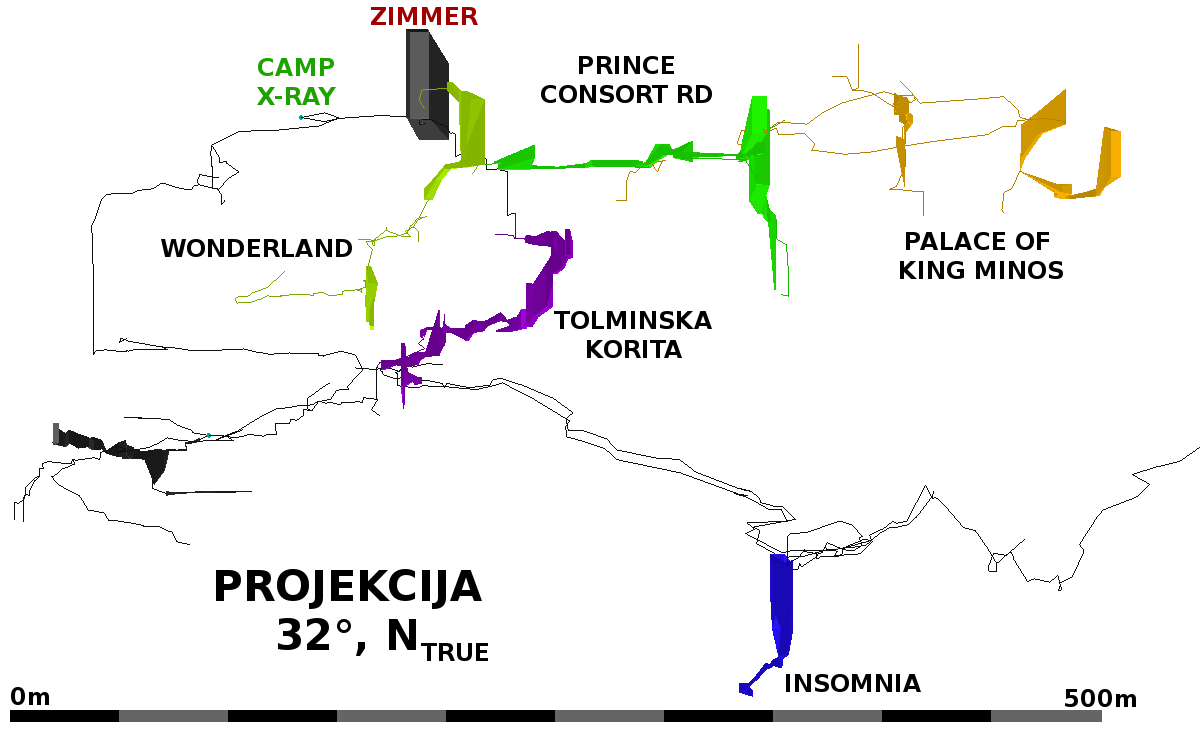
\includegraphics[width=0.85\columnwidth]{2010/2010_deep_vrtnarija_colour_coded_inverted_labelled}
\caption{Colour coded diagram of new cave discovered \& surveyed in 2010 in
Vrtnarija.}
\end{figure*}

\section{Expedition Findings}

The initial effort of the expedition was directed into setting up
underground camp. As the first pushing trips from this underground camp
came back with positive news, exploration based from camp (i.e.~deep in
Vrtnarija) quickly became the main focus of expedition effort. This came
at the cost of further work in bounce trips down Captain Kangaroo
(Vrtnarija, the likely connection region to M2) and M2 / SysMig itself.

The usual surface bashing continued, looking for new cave systems on the
plateau. A revisit was made to the area north of Kuk. This region is
heavily cratered with clear cave development, but the fear is that the
limestone is too broken and chossy for a human sized entrance.

We first visited this region with a serious aim of cave exploration in
2008, and returned in December 2009 on a `winter recce' by a two person
team with ice axe and crampons to identify which surface features were
actively linked into extensive underground systems through the holes
blown in the snow. Several more entrances were identified during this
recce, ones that were likely to be continued to be ignored in the summer
due to their unusual position.

These entrances were relocated this summer, but no new descents were
made.

\subsection{Leopard --- 1.5 km of new passage}

\begin{figure*}
\centering
\includegraphics[width=0.9\columnwidth]{2010/2010_new_stuff_extended_extraction}
\caption{Extended elevation of new cave discovered in \textsc{TOLMINSKA KORITA} and \textsc{PRINCE
CONSORT} during 2010 Expedition.}
\end{figure*}

Leopard became the great focus of exploration this year. This lead (a
window off Zimmer chamber, now a 15m `up' pitch) had also been
originally discovered in 2001, but the drop that it led to had lain
untouched since then. This was partially due to its loose and muddy
nature, but also that deep exploration had concentrated on good leads
elsewhere (most particularly the lower Vrtnarija level accessed with the
bottoming of \textsc{Big Rock}). This took several sessions of rigging
and gardening to successfully conquer, and is is now named Cheetah
(P35m), because of the sense of having cheated death that it engenders
on passing. There are several windows off Cheetah, which are definitely
promising, although not easily accessible because of the broken nature
of the rock.

At the bottom, it intersects a horizontal, fossil passage, which has
been explored in three main horizontal parts:

Wonderland (heading South) linking into Rolling Stones, Surprise,
Mudstone Traverse, Kamikaze and finally Lost Hopes. Mainly dry with
large breakdown chambers.

Prince Consort Road (heading North) was initially pushed to
\textsc{The Albert
Hall} (from where the \textsc{Serpentine} meander leads off to the
\textsc{It
Will Rain for a Million Years} pitch), bisects three streamways (one of
which was pushed and forms the Esoterica series) and includes
considerable calcite formations.

From \textsc{The Albert Hall} a climb was made into the
\textsc{Palace of King Minos}. This passage is complex, and side
branches have neither been fully explored nor surveyed. The known
passage leads via Minotaur Rift to terminate in the Queens Bed Chamber
where the draught disappears towards the ceiling.

Together this passage leading off from Cheetah has been explored to over
1.5 km in length, and we are sure that more is yet to be found.

A significant volume of air flows through these regions, indicating that
there may be further developments.

\subsection{Wonderland}

Wonderland is the southern-most of the horizontal development, leading
directly off from Cheetah. It was pushed to a small pitch dropping into
a boulder filled chamber, Rolling Stones, which was the limit of the
first exploration trip due to the lack of rope. This chamber is situated
right below Zimmer, about 40m deeper. There is a further, as yet
unpushed, pitch going down between the large, seemingly unstable,
boulders on the floor.

A happen stance crawl behind some boulders led to further drafting
passage (Hidden Surprise), which, after traversing another chamber and
crawl, finishes in a chamber with a massive hole in the floor (Kamikaze
pitch). The passage continues on the far side of the pitch (traversed on
mud along the left wall), however, due to the collapsed ceiling, these
developments are almost two-dimensional (Mudstone Squeeze). The squeeze,
which is filled with interesting fossilised mud formations, was pushed
to the limits of comfort, although it still continues.

Kamikaze consists of a series of small ledges. From the second ledge a
tell tale breeze led to an interesting bedding plane crawl pushed upwind
but still untouched downwind. The pitch was bottomed (Lost Hopes),
wherein an inlet was followed down a 10m pitch to a series of squeezes
and rifts which quickly became tight. There is a ledge halfway down Lost
Hopes, with a perhaps larger abandoned rift.

These three leads (Kamikaze, Mudstone, Lost Hopes) are of interest as
they now form the most Easterly extent of Vrtnarija at depth, seeming to
`spear' through the large N-S geological feature that contains the
majority of the horizontal passage.

The whole area of Wonderland is extremely dry, quiet and rather spacious
in its scope. It is particularly reminiscent of the higher level passage
in the Easegill system, Yorkshire.

\subsection{Prince Consort Road}

Prince Consort Road is the passage going north from Cheetah. Several
streams intersect it and some formations have been found there. The
discovery of stalactites covered with helictites proved particularly
exciting! The passage leads to a small boulder choke which was easily
surpassed and led to a large chamber (the Albert Hall). Before the
Albert Hall, three apparently unique streamways have been found:

One intersecting the passage along a traverse (water chokes into boulder
floor), then around a small chamber at about halfway to Albert Hall, on
a corner of the main massage approximately 2/3 of the way to the Albert
Hall a small rift to the east, and a nice white-sanded water inlet to
the west. The latter leads to an unpushed pitch under the main passage,
there is a cairn and note mentioning the lead. Of these, only the second
has been pushed, into the Esoterica series. Strangely this wet, tight
rift has only been visited once during the expedition, even though it is
still going!

In the Albert Hall two streams enter the chamber from on high (the
ceiling was measured as being over 30m up, by laser disto) and join into
a rather beautiful spacious vadose streamway (The Serpentine).
Serpentine was pushed and leads to another split pitch (It Will Rain for
a Million Years \textemdash{} pushed during a continuing flood pulse).
At the bottom of It Will Rain pitch the stream continues and has not
been explored.

\subsection{The Palace of King Minos}

North from the Albert Hall a muddy climb lead to The Palace of King
Minos. This passage and its continuation (The Minotaur Rift) has some of
the most beautiful formations found on Migovec to date, in particular
fine walls of calcite, gypsum and aragonite crystals, mud formations and
weird soot encrusted floors. The Palace has a labyrinthine nature with
several passages leading back to Albert Hall, the largest loop of which
was named Ouroboros

The passage has a classic large phreatic lozenge shape, with some parts
undercut by fossil vadose passage. Near the start of the passage a
significant breeze blew through a small hole. This was enlarged and
found to lead to a small phreatic tube which bizarrely led into an
active vadose streamway (Povodni Mo\v{z} \textemdash{} Water Nymph).
Povodni Mo\v{z} has been pushed upstream to a large active aven (and
smaller dry parallel shaft), and downstream to a sump (approximately
2mx2m in size in the corner of a small chamber and taking the small
flow) and has hence been derigged.

Continuing along the main Palace passage several horizontal tubes have
been explored which lead back into the main passage, though not all have
been entered in the survey. Eventually the main route leads to a high
and wide rift (Minotaur Rift \textemdash{} 20m high, 60m long) beyond
which the best formations are to be found. This passage has a few
interesting leads in it: a high, dry, circular, muddy window to the
right of the passage near a tiny inlet, 2 small tubes leading off the
main passage which both need a little mechanical persuasion.

The chambers beyond Minotaur Rift are spacious and display massive
amounts of crystal formation on all available surfaces --- there is
white `popcorning' almost everywhere, with regions of more intricate
needle and feather formations. The chambers decay into a crawl, which
almost unbelievably is over a smooth calcite floor. This leads to a
classic boulder choke gallery (choking at the end). On the left a small
boulder choke climb leads to the Queens Bed Chamber. In this large room,
the draught appears to disappear up towards the ceiling - both ends of
the chamber are potential climbing projects (\textasciitilde{}+20m).

The region is extremely reminiscent of Ogof Ffynnon Ddu II in Wales.

\section{Tolminska Korita}

This lead of Zimmer chamber had been discovered in 2001 but had lain
unexplored until last year, when the first few pits of the active
meander were pushed to a larger pitch. Korita developed into cascades of
active pitches (Black Knight series) to a duck. The duck was soon
bypassed by a 5m free climb into old phreatic level.

The passage beyond soon diverges into two continuations:

\subsection{Sidewinder, Crack in Time}

The higher dust filled dry phreatic level (Sidewinder, Crack in Time)
connects into \textsc{Envy} in the low level via free climbs and two
small pitches. It is not particularly surprisingly that the `Crack in
Time' was not explored from below, as the connection is made by a long
body-sized crawl above a thin (5 cm) crack connecting to known passage
(Envy), which happily pops out at the top of a obscure 3 m free climb.
Connecting into a 2004 era permanent survey station, Korita now forms a
second loop in Vrtnarija, forming Vrtnarija into a figure-8 shape with
Friendship Gallery at the waist.

\subsection{White Bishop, Stalemate}

The active streamway descends two 10-15 m pitches connected with a
spacious meander incorporating free climbable cascades, before ending in
an impassable rift (-662 m).

This water disappears into `blank mountain' on our survey, but would
require considerable effort to progress, and Korita was thus derigged.

\section{Roaring Floor Tease (Muddy Window off Happy Monday)}

This was regained by bolt climbing from the bottom of Happy Monday to
regain the Muddy Window. The climb in the mud chamber was made, but
quickly led to a large boulder blocking the way. A tight rift taking a
large draught was left unpushed. Progress is believed to require
expansion.

Similarly the traverse to an inlet on Falls Road, and the continuation
of Falls Road itself was left unpushed. A small dig was made in
Friendship gallery beyond Prima junction, which led to a small unpushed
pitch above a stream.

\section{Deep Leads (Below \textsc{Big Rock Candy Mountain})}

\subsection{Insomnia - Republika Streamway}

Last year a `written off' streamway (Republika, leading from Red Cow)
was found and pushed upstream to an aven fed watershed, then down the
other limb to a rift pitch.

With the promise of being one of the deepest points of the cave a return
in 2010 was obligatory. The pitch was found to be 41m and was pushed
down a continuing active rift (Insomnia). The end is now only 4m higher
than Colorado Sump (the deepest known point of Vrtnarija). Since the
limit of exploration is above a small 4-5m pitch it is understood that
in 2011 this will inevitably become the deepest passage in the system,
and the signs are good for continuing development of depth. The end is
802m below the entrance of Vrtnarija, but the M2 (Kakna Jama) entrance
is 75 m higher still, and a connection between the systems would make
this point -877m deep overall, with potential for further depth
extension.

\subsection{Balamory}

A return to Balamory was thwarted by lack of rope of the exploratory
party (one more pitch than expected on route), but the team made good
use of the trip to the depths by recovering the camping mats from the
deep 2004 camp (The Fridge, near Cactus Junction), and prospecting for
other leads with some success.

\section{Original Exploration Stories}

\subsection{Pushing Insomnia}

I had travelled down to T'min to clean and get over the cabin fever that
develops over the weeks of life on the Plateau. That night, after a slap
up meal and a few bruskies, Jan arrived and we had a great evening of
beer and bullshit. After the beer, we passed on to the whiskey and the
bullshit got increasingly epic. ``The leads at the bottom of Red Cow are
going to make GW deeper'' I told Jan ``the next pushing trip will
definitely do it''. So after walking up the hill having dinner and a
little too much to drink at the bivi we set off for the night train.

Soon enough we are at camp and decide to keep going down, looking to
continue pushing the Republika lead. I must admit it took a lot of
strength not to push the leads that were already multiplying at the I
knew the way to Red Cow, having been there with Dan a few days earlier.
We soon got to the junction and followed the water upstream. Nice
caving, I start feeling the all familiar excitement: here come lots of
km of fresh cave!

At one small pitch I turn around and find Jan has disappeared. I turn
back to look for him and find him wandering in the wrong direction
towards the sump. Apparently he had fallen asleep and started wandering
off route. Shit maybe we are too tired for this? Meh! We get to the
pitch head for Republika, which I must admit is rather God forsaken and
wet and awful. We drop the pitch, I get the drill out and start rigging,
brain totally disengaged. As I am rigging I can feel the batteries
getting weaker and weaker. I guess there were a few too few bolts at the
bottom of the main drop and maybe some of the pitch heads could have
been a little neater. It certainly helps to cave with a tall bastard is
all I can say :D.

We reach the bottom of the main new pitch and it's a rather God forsaken
wet and damp place. The water keeps going down along some immature
passage. We follow the water, noting at least one unlikely but unchecked
possible side passage. A few hand lines are placed here and there and
the drill battery finally dies. Just as well as the last pitch we get to
looks like a right nightmare: really tight pitch head etc. By this point
we realise it's super late and we are almost certainly going to miss our
callout. Time has gone in a blur, we are probably not 100\% there
mentally to be honest. Still might as well survey out.

The way out is not very remarkable. We bump into Tetley at the top of
Big Rock. He is not too worried, but apparently Gergely was hoping we
were crumpled up in a heap somewhere so he could come and rescue us.

\attrib{James Kirkpatrick}

\subsection{More Horror with Jan.}

The next night we get up and decide to do some pushing. The whole day is
marred by the fact that - once again - we promised not to push the
obvious continuation from Albert Hall. So we decide to have a random
bimble around. We try looking for alternative ways around the Albert
Hall. No success. Somehow we end up pushing a lead from the right of the
passage leading to the Albert Hall (right looking towards the Albert
Hall!).

The passage is small and bends under the main route. It is wet and
rather grotty. We drop a pitch or two of utter horror and eventually
turn around. Surveying out is awful. The book gets wet, my fingers are
too cold to hold the
instruments\footnote{The survey data had to be 'corrected' to avoid the survey self-intersecting due to backwards legs.}.
It sucks majorly. At least the passage gets a cool name: Esoterica. O,
and no-one has pushed the pitch where we stopped!
\footnote{Esoterica was not revisited until 2012, where a broken bolting driving prevented any additional pitches being descended. It remains a lead.}

\attrib{James Kirkpatrick}

\subsection{Happy days with Jan.}

On our last day together we went looking around the amazing passage that
we politely left for Dan and Izi. We smashed our way through the
entrance of what would become Po Vodni Mos, we looked at the Queen's bed
chamber, we pushed down some random tubes at the sides of the main route
(has anyone ever surveyed these I wonder, one of them went!). All in all
a super chilled day. No surveying and no water. And then we got back to
camp, watched some videos and drank a lot of whiskey, Happy Days!

\attrib{James Kirkpatrick}

\subsection{Balamory}

When James and I went to have a look at the bottom of Balamory on the
first day of our one-noght camping trip, we didn't make it to the target
as an unexpected first pitch used up too much of the rope that we had
taken with us.

However, as well as airflow going towards Balamory, there is also
airflow in the main passage above, beyond the point where the hole down
to Balamory leads off so here are two leads in that area there that are
worth looking at.

The upper lead \emph{does} need some way of climbing across a pit to a
ledge covered in loose crap (maybe a bolt traverse round one of the
walls, though I can't remember how much good rock there was in that
area. Subsequent email exchanges on the subject do seem a bit vague as
to exactly what was done, and whether the upper passage had actually
been boldly examined or not (Clewin was bold somewhere round there, but
it wasn't certain where), but anyone going to potentially move/split the
boulder down Balamory (I think it was supposed to be down the third of
the three possible `second pitches') down should also probably plan to
look at the upper passage continuation, especially if they have a
drill/bolts to help with climbing/traversing belays.

On the way back from this little trip, after grabbing some stashed
karrimats from the old camp, that the black black hole across Big Rock
was noticed.

The next day, James and I went to the new stuff below Leopard/Cheetah,
but since we were doing a push-then-out trip, rather than going to the
far end of the `half' where most of the action was, we went in the other
direction from the pitch bottom to do some work relatively close to
camp, carrying on where Gergely+???? had left off at the Hidden Surprise
pitch.

Gergely had dropped the first section of the pitch to an obvious ledge
and followed the ledge to horizontal passage that soon died. James and I
were to descend the shaft from the ledge, but it immediately became
clear the drill wasn't working and so we had to resort to spits, with
James bolting while I waited on the ledge.

Fairly soon the bolt (bolts?) was in and James had descended to a large
boulder-covered ledge part-way down the large shaft, where I could
safely join him. Some of the boulders were rather large, with gaps
between them or between them and the wall large enough to climb down and
move around in. While James did the business with the next spit, I
wandered around between the boulders to keep busy. Where the boulders
met the wall, the wall was somewhat overhanging, and from the lowest
easily-accessible place near where I had first climbed down, it was
possible to look between the boulders marking the lower limit of easy
movement and the wall to see a few metres away/down to where the wall
seems to meet the proper floor of the ledge, where there was a layer of
white rock flour, with some potentially human-sized space between me and
it though with no obvious way to get there.

From where I was, looking along the wall `clockwise', it also looked
like there was a space of some sort ahead of me horizontally, but
getting to it didn't look very nice, and after all, I was just in a pile
of boulders on a big ledge half-way down a pitch, not in a classic
boulder choke as such, so there seemed little point doing anything
borderline just to get to a slightly different place in the boulder
pile.

However, just as I was preparing to go back up and see how James was
getting on, I breathed out a large sigh, only to see it get sucked
horizontally away from me between wall and boulders and into the space I
had been looking into, which immediately aroused my curiosity.

To get into the space I could see required going horizontally through a
not-quite-body-sized vertically-rectangular gap with a short (1m) drop
on the other side. After removing all my SRT kit, and doing some work
with a convenient rock hammering edges off the boulder forming one side
of the slot to make the gap wider, and progressively blunting sharp
edges on the wall side as they proved awkward when attempting to get
through, it was possible to slowly and delicately post myself through
feet first and eventually emerge free on the other side.

Turning around, a short crawl led to a wider area under the overhanging
wall, and a view ahead to where the wall/roof sloped nicely down towards
into the floor to leave a wide bedding plane with clearly no way on.
Turning around somewhat disappointed, the main wall, which I had been
looking away from when I had initially turned round, was seen to have a
crawling-height hole in it, which, on approaching, it was clear most of
the draught was going into.

That hole led to a small chamber with a further hole leading in turn
into the side of a walking-height passage with a good breeze running
along it. The draught I had followed initially was clearly just a
tributary being sucked into the main airflow.

I quickly returned to James to tell him of the find, and we decided to
do a little surveying and exploration. We chose the upwind branch which
didn't run a great distance before ending in an upwards bedding-plane
slope ultimately blocked by a large slab in the bedding blocking
sideways movement into what appeared to be a chamber with a waterfall
entering. Capping or plugs/feathers would seem to be needed to shift
this blockage. On returning to our entry point, we looked the other way,
wondered how far the downwind passage went, but left it for someone else
to explore.

We hadn't found a great deal of length, but on the other hand, we had
left a decent going lead, and due to the combination of a misbehaving
drill making waiting cold and dull work and the luck of my breath
showing there was something worth looking at, had ended up finding quite
interesting passage in what must be one of the most unlikely of
situations.

Thinking partly of the initial nervousness with which I had slowly
posted myself between the boulders and the wall, but mainly of the
immense luck we had had with the draught, Kamikaze seemed like the
obvious choice of name for the discovery.

\attrib{Dave Wilson}

\section{M2 --- Kavkna Jama}

The JSPDT organised a trip based at the mountain hut at Kal on 2nd
October 2010. The terminal rift was enlarged to gain a $\approx$ 20 m
pitch and a larger, undescened (due to lack of rope), pitch.

A return trip three weeks later descended the pitch and found it to be
$\approx$ 60 m. The cave closes immediately, with a tight rift taking
the water and a slightly larger abandoned rift also offering potential.
It draughts strongly.

The M2 cavers returned in thick fog, following their footsteps through
the 10 cm deep snow. With the coming winter Migovec is effectively
closed for exploration until summer 2011.

\section{Exploration Outlook}

In all, 2.2km of new cave was found during the 2010 Vodna Sled
expedition, taking Vrtnarija to 8.776 km.

We are in the extremely fortuitous circumstance where we finish the year
with considerably more leads in the Migovec cave systems than we started
with. The Vrtnarija camp was derigged with the certainty that we will be
back next year camping in the same location. Gas cylinders and cans of
fish were left sealed in Daren drums with a rock of carbide to keep them
dry, the carry mats and tents were left standing to air, and we have a
considerable armoury of rope brought back from the pushing fronts
waiting for the 2011 team.

The work by the JSPDT in the Autumn has \texttt{opened up} M2 once again
and brought the possibility of forging a connection back to the table.

The pushing of the Republica streamway (now Insomnia) to within a few
metres of the maximum depth of the cave has reawakened the possibility
of further depth extension to Vrtnarija. Expedition members have mooted
the possibility of establishing an additional 2-man `deep camp' to
benefit pushing trips in the lower reaches of the cave, particularly any
revisits to the far North end of the system.

\section{Migovec's Long Term Prospects}

It has been a recurrent discussion in our club as to when we will run
out of new cave to discover in Migovec. Almost all of our fruitful
exploration has taken place within a single square kilometre of the flat
topped mountain.

Migovec, being part of a mountain chain that is the first high altitude
interruption to moist air from the Adriatic, receives an extremely
significant level of rainfall. This summer, Jaka Ortar, a Slovenian
geographer, recorded 210cm of rain on Migovec in 100 days (28th July-3th
November) with his network of rain gauges. However we have never found
any large rivers underground --- the known cave can only account for a
tiny percentage of the total drainage for the plateau.

Our current hypothesis is that there is no \texttt{master system}
gathering the water, but instead a complex hydrology induced by cave
passage intersecting the underlying (as yet, unvisited) band of
Cretaceous shales.

For all Vrtnarija's complexity, the entire cave can be fitted into a
slab of limestone slanted at 66 degrees and just 1000x150x1000m.

Certainly, as long as we can continue to find entrances through the
frost shattered and heavily cratered surface, there will be enough cave
in Migovec for decades more of exploration.

\section{Underground Logbook}

\section{Found in `AggregateofMig2007-2010.doc' : Jarv Typed up?}

Camp X-Ray Logbook: After about 6 hours of caving, finally made it down.
Met Gergely \& James on he way down as they were leaving the cave. Last
bolt before camp is horrible = needs rebolting / rerigging. 15cm lower
would be awesome. Built a tent at teh camp. Required some stone
movement. Mike got water, me \& Jarv built tent, kate = smoking. NEED
WEED! Should have thought about it before. Listening to Massive Attack
and getting Raptured. Oh yeah! Kate setting up sleeping space, Jarv went
to get more water.

Camp is getting established, looking forward to Worms World Party. Mike
= Cooking. Weed is really a missing resource. So far so good. About 5
metres from camp is a hole with water in it = able to hear, quickly got
established as peeing corner, hope its not a lead\ldots{} Nick

23/7/10 Nice snooze - super warm. Nicola snored like a trooper - just a
few minutes into the classic Black Adder session. Broken sleep -
particularly as Nicola got up for X2 piss. Awoken @ 10:30AM by the
beasts crawling up towards our pits. Tetley \& Myles rustled up some
hot-choc then wandered off down the continuing passage.

23.7.10 - 2:10pm MD + Tetley Entered Gardener's World
\textasciitilde{}6:20am. Made our way through, re-rigged zimmer on the
way. Arrived at camp at 10:30am + awakened JV, Mike, Kate + Niko.

Wandered around friendship gallery for hour or two. Found nice lead,
will investigate later. Sleep now.

23-7 2:20pm

It's good to be back in a sleeping bag at Camp X-Ray - seven years since
the last camp here. It's very comfy. I like the tent - some things don't
change though, Blackadder on the sound system, smash + tuna etc.
Hopefully we'll get some good pushing in tomorrow! Tetley

23-7 6:20pm James and Dan arrive for a quick visit before heading off to
push the muddy window 8:20pm Andy + Gergely arrive - I ignore them! Tet

23-7 10:30pm Fucking body won't fall asleep! Must have only had couple
of hours at most since Dan arrived\ldots{} Gergei + Andy turned up at
8ish + now, they have checked our Leopard a little. Tetley's bodily
functions are out of control! May bring some corks down for his
digestive tract next time. Anyway, now for some food + tea + hopefully
can stay awake till bedtime at noon! Myles.

23-7 11pm Myles and I share breakfast / dinner with Gergely + Andy. Fine
food! (Ed: Believe this was Tetley)

24-7 12:20 Breakfast with Tet \& Miles. Dan \& I will visit the lead we
killed yesterday (Muddy Window) \& survey it, then to Red Cow. James K

24-7 1:30pm MD Back in Camp for 2nd night. Pushed Tolminka today, good
lead, surveyed \textasciitilde{}8am. Some nice pitches. Covered in mud.
Listening to strange foreign music.

24-7 2:05pm Great push down Korita today - 8 bolts, surveying etc. IT'S
GOING GOING GOING\ldots{} GO THERE! (But try and avoid rigging future
pitches in or near the water\ldots{}) Andy + Gergely have left to push
Leopard - James + Dan to survey Muddy Window and then go for a jolly
below Big Rock. I've had a great day - thanks Myles. Time for a decent
seep. Tet

23:20 24/7/2010 James + Dan return on a high! 9hrs good kip in bed - I
feel good! forgot to say I had a shit yesterday\ldots{}. Tet

\chapter{2011 --- Izgubljeni Raj}

2011 was another great year deep within Tolminski Migovec. The weather
was horrendous --- we even had snow! But the cave kept on going. We
found over 2.2km of new passage all below -500m in depth, and took the
cave to a new deepest point of -888m. All of the exploration took place
during underground-camping trips based at X-Ray (Vrtnarija, -550m), with
the keenest of expeditioneers managing a total of around seven nights
underground during the four week expedition.

\subsection{Introduction}

Between 15th July and the 15th August 2011, Imperial College Caving Club
had twenty members participate in the Izgubljeni Raj 2011 expedition to
Tolminski Migovec, Slovenia. The aims for this expedition were the
continued exploration of Vrtnarija, where considerable efforts in 2010
had led to the discovery of 2.2 km of mainly horizontal passage, all
below 500 m in depth. At the start of the expedition, Vrtnarija was 8796
m long and 807 m deep.

This summer we had less manpower than last year, but were still
attempting to set up a similar four-man camp at -550 m and carry out
deep pushing. Our exploration continued routes which were diverse in
direction from camp---soon we were taking many hours just to travel from
camp to the pushing front and back.

As a result of the reduced manpower and the considerable demands that
exploration of Vrtnarija was making on our time, we unfortunately did
not manage to contribute towards the exploration of Kavkna Jama and the
attempted connection of the Migovec and Vrtnarija systems.

Our efforts were considerably hampered by the weather. We had the
wettest summer we've ever experienced on Migovec. We only very rarely
had sunny enough periods to dry our caving equipment and clothes. A
particularly memorable rainstorm of 48 hours near the beginning of
expedition was rounded off by a heavy snowstorm -- the first we've ever
experienced in 15 summers on this mountain!

For two periods of 36 hours, underground camp was effectively cut off
from the surface by high water levels in the cave system, making some of
the pitches impassable. Thanks to the quality, warmth, provisions and
size of underground camp this wasn't a major problem as exploration
simply stopped and the explorers got a lot of sleep instead. Certainly
underground camp was a more pleasant environment than the windswept,
rain lashed and barely above freezing surface of the mountain.

In all we discovered 2229 m of new cave passage taking the cave to 11025
m long and 888 m deep. All these extensions have been made at depths
greater than 500m, on multi-day trips based at an underground camp.
Vrtnarija now has the vast majority of passage, over 8 km, at depths of
greater than 500 m.

\section{Cave Discoveries}

Our major cave finds this year can be considered in three separate
developments within Vrtnarija:

\subsection{The Serpentine \& Let na Drugi Svet}

An active streamway, named the Serptentine, led off from a large chamber
(The Albert Hall) discovered along Prince Consort Road. During 2010,
this was pushed to -621 m (Will It Rain, for a Million Years?).
Exploration in 2011 continued along this active meander.

The initial exploration (Round Pond) descended a 2m climb down leading
to an oxbow and 4m pitch. The following trip traversed out along a crack
in the ceiling to avoid falling water down a 10m pitch (Longwater) which
entered a chamber (also Longwater) with significant iron deposits (in
the form of heavy \textasciitilde{}4cm thick plates of dark mineral in a
vein within the limestone), and a considerable number of orange-stained
straws and stalactites.

The boulder collapse in this chamber was bypassed by a squeeze between
boulders on the right which entered a crawl-way which soon refound the
water flowing from beneath the boulders. A 4m pitch was reached where
the bedding plane appeared to intersect a joint. A 3m diameter
apparently rather deep pool is present below this pitch. Passage
continues in vadose development with the water, which entered a small
chamber with a set of cascades (cascade chamber). There is also an
apparently phreatic connection between high up in the roof of this
cascade chamber and part way up the 4m pitch.

The cascade chamber is rather complex in structure, the cascades falling
into a large \& deep 4x2m pool. This water flows down a short rift and
immediately tumbles down a \textasciitilde{}8m pitch (Duffers Drop)
which leads via two freeclimbable cascades (requiring very careful
maneuvering near to the water) to reach a wet inlet on a large pitch
(Drink Your Own).

Behind the large pool in cascade chamber there is a dried pool with
haematite deposits and the start of a phreatic crawlway (Rotten Row),
which is hidden from view unless you're crouching next to the dried
pool. This crawlway leads to a short pitch into the dry end of the
rift-developed Drink Your Own pitch.

The cascade chamber also contains a rock bridge which can be used to
traverse over the chamber into a dry scalloped shape alcove and so avoid
climbing the direct 2m cascade to the pool.

The maximum depth reached was -688 m. Our surveys indicate that the
current termination, at a large wet pitch with two accessible pitch
heads (via Duffers Drop, or Rotten Row), is very close to the Republica
chamber at -723m, where two streams enter from the ceiling and split.
Exploration was halted by the wetness of the pitch, which will require a
considerable effort in bolting to rig safely. Drink Your Own is a pitch
which has developed in a perfectly straight rift (probably fault
controlled), with two streams entering the rift from opposing
perpendicular directions (i.e.~perpendicular to the rift direction of
the pitch), one of which is the Duffers Drop water which we have been
following continuously from the start of the Serpentine in the Albert
Hall.

The Serpentine rope was derigged back to camp to avoid water damage
during winter.

The Serpentine water flows continuously from the Albert Hall chamber to
enter Drink Your Own via Duffers Drop. The water entering on the
opposite side of this large rift pitch is considerably greater in volume
and the source is unknown.

Below the first pitch in the Serpentine, a climb was made to access Let
na Drugi Svet (Fly to Another World), which via a series of digs and a
21m pitch led to a large active meander Krt Kova Dobra Dela (Little Mole
Done Good), which is has been pushed both upstream (to +19 m) and
downstream (to -23 m) and is ongoing. It is possible that this water
forms the larger of the streams that enters Drink Your Own.

212 m of passage was found below It Will Rain, and 252 m in Let na Drugi
Svet.

\subsection{Insomnia}

Insomnia is the continued exploration of a descending streamway in the
`deep' level of Vrtnarija off Red Cow Roundabout, which started with
Republica in 2009 and was left with an active streamway at -802m
(Insomnia, 2010). Two pushing trips (Daydreamers) followed this stream
down a series of small (5-15m) pitches. The last trip saw this stream
disappear into a narrow, too-tight, rift. A bypass was sought via an
abandoned bedding plane level (Penguins Egg), which gained the head of a
chamber in which the noise of falling water could be heard.

The descent and exploration of this chamber (Winter Journey), found that
the loud stream noise could be heard through a too-tight rift formed in
a bedding plane with the characteristic -70 degree dip of the passages
near the sumps in SysMig. This rift was also issuing a draught, which
was followed along the inclined bedding plane (heading North) through a
series of muddy squeezes to where it disappeared into an immature rift
in the roof. It is hypothesised that this could be the water-driven
draught return from a sumped section. The chamber had considerable thick
grey silt deposits, with unusual silt stalagmites on the boulders, which
may be evidence of a sump backing up.

The bedding plane was pushed in a northerly direction for circa. 20 m.
This is in the direction of the hypothesised dip of the mountain's water
table, and so it is possible that continued pushing or digging of this
bedding plane may lead to a sump bypass.

Exploration was carried out by trips that started on the surface
(confirming good weather for the day), went to the bottom, explored and
then returned to underground camp. This was due to us being extremely
concerned about the flood response of this new part of the cave. The
pitches are active, and due to a combination of the unavoidable cave
nature, and `exploration' rigging, they are wet even in moderate
conditions.

The 2011 exploration of Insomnia found 294 m of passage and took the
cave to a new maximum depth of -888 m. The pitches were left fully
rigged as the intended last pushing trips did not occur due to a
multi-day rain storm near the end of expedition.

\section{Kamikaze}

Kamikaze is a subtle route through the boulders on a ledge part way down
the pitch to Lost Hopes in Wonderland (the name given to the chambers
developing South / South East from Cheetah). The original explorer (DW)
was making good use of his time while hand bolting down the pitch
continued, and the key squeeze through the boulders was only found when
the condensation from an exasperated sigh was noticed to disappear
sideways!

The sandy crawling passage was originally pushed upwind, to eventually
reach a boulder blockage in a spacious bedding plane beyond which a
large sound of water can be heard (Kamikaze). There is enough space in
the bedding plane to dispose of boulder fragments, if it can be reduced
in size, and is an obvious future dig target.

This year we pushed downwind, almost instantly discovering a large
chamber (Red Baron) and a bolt traverse over a pit to reach a large
(\textasciitilde{}6m diameter) ascending (at almost exactly 30 degrees,
in a straight line for 140 m) phreatic level (The Throne Room). This
terminates in what appears to be a cross rift intersecting it, making it
a hammer head shape in plan. There is a 6 m undescended pitch at the
end, and the possibility of a traverse across this pitch and a
continuing crawl way.

Midway along this phreatic tunnel, a climb was made (Serenade) following
the draught through a window and into a parallel piece of passage now
descending (Amazing Grace). This continued with large sections of
passage separated by short boulder chokes where the floor raised to
reach the roof (Magic Dragon), eventually reaching a large and extremely
muddy pitch.

This pitch, Stuck in Paradise (P69m), took three pushing trips to make a
successful descent, and was conquered by the use of an electric drill
and rawl bolts. The rock was too poor, and the pitch literally too muddy
to make effective hand bolting possible. The pitch was formed from a
series of chambers through which a complicated SRT route was found.

Below this pitch, the route split with the discovery of two extensive
horizontal levels:

Lost Miles (originally East Links) is a comfortable walking phreatic
passage of 2-3m width, decorated by plenty of crystals, but which does
not take a significant amount of draught. Exploration was blocked by a
boulder choke after 270 m, which was dug, and nearly passed, this year.
After the boulder blockage, the passage seems to continue with a similar
dimension. There are white crystals (we believe Calcite and Aragonite)
present, but no stalactites. This termination is now the most Southerly
cave passage in Vrtnarija.

The Penitence crawl (originally Knee Killer) takes the draught to a
boulder choke, and includes some clean white stalagmites (the first seen
in Tolminski Migovec) and stalactites. The entirety of Penitence is
crawling in passage with a maximum height of one metre. Midway along
Penitence a boulder choke is passed, with a collection of approximately
half a dozen white stal columns 20-30cm high. Penitence ends in a
boulder choke, which was passed to lead to `Salvation', which ends in
two ways on. The first branch of passage ends at a sandy dig with no
draught; the other is (what appears to be) an easily passable squeeze,
at the end of an ascending passage, with a howling draught. One can hear
a considerable roaring at the squeeze which is possibly water.
Exploration was halted at an open lead by lack of time, after 349 m of
passage from the bottom of Stuck in Paradise. From the start of the
Serenade climb, development to the current end of Penitence is almost
perfectly South-East in direction and 500 m in plan length.

Until the discoveries this year, Vrtnarija almost exclusively resided in
a band of rock less than 200m wide and inclined at 70 degrees. Almost
all the horizontal development was confined to `North-South' development
(actually 330 degrees true) in this band. The new phreatic levels off
Kamikaze have developed hundreds of metres to the South and East,
seemingly unconstrained by this geomorphic feature. They have taken the
actively pushed cave passage into entirely blank mountain, and
underneath the massive drainage basin formed by the Kuk-Razor valley. As
of yet, this passage has been entirely dry, but with a seemingly
increasing draught.

Wonderland, and the Kamikaze extensions, were left fully rigged as this
area is almost totally dry. The exploration front is now a considerable
number of hours of caving from camp, and the lack of accessible water is
a logistical difficulty in staying hydrated. However, this entire region
discovered so far completely weather independent.

In total, 1.383 km of passage was found in the continuing exploration of
downwind Kamikaze.

\subsection{Other Leads}

A choke near camp, at the end of Friendship Gallery (Lower Pleasures),
was dug and passed to a 28m pitch (2nd Time Lucky) leading to continued
small passage. 88 m of new passage has been found. It is hypothesised
that this passage may be the natural continuation of the older
Friendship Gallery phreatic, before the vadose development of Big Rock
occurred.

Big Rock, the 74m pitch at the end of Friendship Gallery was known to
have a window from it's first descent in 2003. Recent inspection with
modern high powered lights have revealed that it is more that we are
descending in the side shaft, and that the main chamber is still to be
gained! The chambers are separated by a wall of rock about 20m off the
floor of the known pitch. A considerable volume of water can be heard
falling down in this other part of the pitch. We have no idea where this
water goes or where it could be coming from, though it was hypothesised
(in 2003) that water from Big Rock may combine to form the Soda Stream.
A drill battery was expended in starting a high traverse in the process
of gaining the window. As Big Rock has developed in a long rift and we
abseil down the near end, the horizontal distance to be gained is large,
perhaps 30m.

A bolt climb was made in the Queen's Bed Chamber, using an electric
drill, 8mm rawl bolts and a Raumer `stick-up'. Progress was halted by
the muddy layers in between the bands of good limestone. In order to
reach the hypothesised continuation of the phreatic passage, a further
10 m of climb is needed with a solution to this technical difficulty.

A bolt traverse was made to one of the windows on Cheetah, and was found
to be a small abandoned inlet cascade.

The oxbow just at the beginning of Prince Consort Road (just beyond the
roped traverse past the inlet, on the right) was pushed to a tight
inactive rift that leads upstream about 30 m and terminates in a small
chamber. Further climbing upstream is possible. This was not surveyed.

Windows in The Albert Hall and Minotaur rift were inspected, climbed,
and found not to continue.

\section{Prospect for 2012}

The pitches in the entrance series to -550m were derigged with the ropes
left coiled in situ and the metal removed to the Bivouac on top of the
mountain for cleaning and upkeep. The underground campsite was readied
for winter with small reserves of food and fuel being left in Daren
drums, the tent being flipped upside down and the roll mats stood up to
dry. Rope derigged from the Serpentine and other pieces used temporarily
for exploration have been left at underground camp for use in future
years, along with a dynamic rope for climbing purposes.

With sufficient caver manpower, we intend to establish a similar deep
camp in 2012 and continue the deep exploration. Though we have
considerable transit times to reach our current pushing targets, the
diverse direction in which they are going suggests that at this point
Camp X-Ray is a good a campsite as any other.

We are keen to extend our knowledge of the hydrology of the plateau, and
feel that more extensive dye tracing with a visible agent will be the
best route to understanding both the passage of streams within the cave,
and (with larger quantities of dye) identify the resurgence. Due to the
sensitive location of Migovec in the Triglav national park and as the
potential drinking water source for a considerable number of local
settlements, this has to be carried out with full support and agreement
of local government agencies \& population. As such, putting together a
scheme of work \& organising permission may require a considerable
amount of time.

\section{October M2 / Kavkna Jama}

A weekend trip with the JSPDT in October to M2/Kavkna Jama brought back
245m of survey data from discoveries over 2009-2011, adding 100m of
depth to M2 and bringing the closest approach between Vrtnarija and
Kavkna Jama to 4m (with a +- 30m estimated error of the 1.4km unclosed
loop). The lead ends at an easily dug mud floored bedding plane, leading
off into a tight rift, with an extremely strong draught. The trend of
the cave passage is Northerly, towards the Captain Kangaroo area of
Vrtnarija. Even if M2 misses the closest point, Dark Tranquillity, it is
hoped that it will intersect another of the Captain Kangaroo shaft
series at this depth (Olympic Rift, Dangermouse).

\section{Contributed Stories}

\subsection{Attempted rigging of Big Rock alternative, 2011}

Dave and Jon set off for to try and rig to the window seen across Big
Rock the previous year. Attempting to start from the top, Dave bolted
leftwards from the top, slowly, slippily, and still in the draught from
the approach passage, but after a long time spent placing only 6 bolts,
had only reached 1/3 of the way down the initial slope, getting into
increasingly poor rock as he went.

Giving that up as a lost cause, D and J both descended Big Rock to have
a look from lower down. It became rapidly clear that that would have
been the right thing to do in the first place, with, it seemed, only a
few bolts needed to reach and then protect a ledge route around to the
bottom of the window. It also became clear that the window wasn't a
window at all, but a seemingly complete parallel shaft, only divided
from the bottom of Big Rock by a \textasciitilde{}10-15m high wall at
the bottom, with no visible division any higher up - the `window' seen
had been an illusion caused by looking across from high up Big Rock,
where an intervening overhang on the right hand wall had played the part
of the top of the window. It wasn't obvious how far down any parallel
shaft might go beyond the wall, since all that could really be seen from
any suitably high vantage points was blackness, but it did seem that the
parallel shaft was a good size in terms of diameter, maybe larger than
big rock itself.

On arrival at the bottom, the dividing wall was examined from below, but
no easy climbing routes were seen. A clutch of crabs and hangers were
retrieved from between the cobbles near the base of the rope, presumably
dropped by someone in a previous year, but still in very good condition,
so the day had not been entirely wasted.

\attrib{Dave Wilson}

\subsection{Setting up camp: my first time in Vrtnarija!}

It was my first ever expedition and after three(?) days of carries in
rain and clag, I was eager to experience Vrtnarija and alpine caving
firsthand. So when talk turned to plans for setting up underground camp
I made sure I was around for the conversation! It was eventually decided
that a team comprising myself, Jarv, Jan and Myles would finish rigging
down to camp, set up camp and spend a night there before coming out the
next day.

The morning was then spent on final preparations: packing the camp
tacklesacks, sorting out our provisions, grinding black pepper and
packing a cheeky set of survey instruments and bolting kit `just in
case'. Making our way across the plateau to the entrance, I was
admittedly feeling a little apprehensive. I'd never been that deep
underground before and had heard stories about the slog out from camp.
Was I overreaching myself by going down to camp on my first trip? I
trusted myself to make it out though, so it was with an air of
anticipation that I followed Myles into the cave.

Jarv went ahead to rig while the rest of us followed, each encumbered by
at least two bulky tacklesacks, stuffed with sleeping bags and assorted
camping equipment. We met Tetley and Jonny in the Urinal series, on
their way out from Tetley's traditional Mig fresher initiation to
Pico/Swing/Tessellator.

We made steady progress towards camp, chatting while waiting for Jarv to
rig, with Myles telling me about the pitches and where to look out for
loose rock. I like caving with old Myles. He exudes an aura of
confidence and competence. Whether that is true is another point
entirely.

Finally we made our way down Zimmer and through Friendship Gallery
to\ldots{} Camp X-Ray! The overturned tent, courtesy of DanG from last
year's derig, greeted us. We set about making the camp home: collecting
sand to cover the mould which had multiplied in our 11 month absence,
building the sleeping platform of rocks, and setting up the beds of comf
and sleeping bags. I was introduced to the delights of underground
cuisine and the luxury of clean, clean, fleecy comf to wear. Less
glamorous perhaps was having to piss into the same resealable bag as
Myles (I think? Check UG logbook! Or maybe this was in our
tent\ldots{})! I slept well that night.

The next morning after a brew Jan and Jarv decided to have a cheeky push
in Serpentine before heading out, while I was to familiarise myself with
the cave with Myles. We pottered about Albert Hall and its various
branches before finally heading down Serpentine to say hello to Jan and
Jarv. We turned around at the bottom of It Will Rain, the 600m of ascent
on our minds. At this point Myles said to keep going until Fistful of
Tolars as he'd be right behind me. I headed out.

At Zimmer I snagged a sneaky break, deciding to wait for Myles\ldots{}
and I waited, and waited, and waited. Just as I was beginning to get
concerned and go back for him, Myles appeared. Apparently he'd got
confused in Albert Hall and had to try a few passages before finding the
right one back! A bit shaken but otherwise fine, we made our bid for the
surface at a steady pace. The prussick out was actually less painful
than I thought it would be; the never-ending,
one-foot-in-front-of-the-other slog associated with carries was good
preparation indeed!

We emerged to a smattering of rain but felt triumphant nonetheless. I
couldn't wait to go back!

\attrib{Clare Tan}

\subsection{Dream 2 and Penguins Egg}

Morning. The weather was glorious: the sun was shining, and the sky more
blue than white---both rarities on this expedition. I knew there was
heavy rain forecast for the next few days, but for now, I sat on the
outcrop of limestone outside my tent, relishing the warmth of the sun's
rays on my cheeks.

Soon my need for my morning cup of tea became too great to ignore and I
ambled to the bivi, the shakehole that I'd already come to love and see
as home in a scant three weeks. This early in the morning, the bivi was
still relatively quiet as the masses snoozed in their tents, though
Tetley and Dan already had the volcano kettle going---perfect.

Brew in hand, I settled myself onto a `McGowan' (sofas made of dwarf
pine needles wrapped in tarp material) as talk naturally turned to
people's plans for the day.

``Samo's in a pretty bad shape, but I think I've managed to persuade him
to go down with me,'' said Tetley. They'd made plans to push
Daydreamers, an active cascade series at the very bottom of Vrtnarija,
but Samo had been a touch too liberal with the vino the night before.
``I messed up last night,'' he continued, frustrated. ``All I had to say
to him was `Be Ready', before I went to bed\ldots{}''

Sure enough, it wasn't long before Samo staggered into the Bivi, looking
like he'd seen better days.

``Maybe we could go tomorrow instead. I'll be ready then,'' Samo
suggested.

``Nah, I want to go caving today\ldots{}''

Dan and I looked on in amusement. However, when a couple of mugs of tea
did little to alleviate his hangover, it soon became clear that Samo
wasn't in fit enough state to go pushing at -850m in the next few hours.

``Maybe\ldots{}'' Tetley began, eyes taking on that characteristic
gleam. Uh oh; I brace myself. Anyone who knows Tetley knows about him
and his `plans'. I could practically smell one forming in his mind.
``\ldots{}maybe I could go down with Clare today, push Daydreamers, then
you and Karin can come down together tomorrow to meet us at camp, and we
can swap partners? Of course, I haven't even discussed any of this with
Clare yet\ldots{}''

``Yeah, you haven't!'' I nod, eyebrows raised.

Then Samo voiced his agreement, and it was up to me. I hesitated; I'd
already made plans for a fun, relaxing jolly to Pico with Kate and
Nia\ldots{} and Tetley's proposal was a trip of a very different nature
indeed. But the cave was calling. I thought of the lead we'd left in
Daydreamers on our previous trip, the promise of extra depth, the
uncertainty of what we'd find below the next pitch\ldots{} And I was all
too aware, as I am sure Tet was too, that this might well be the last
opportunity of the expedition to push the deep stuff -- the Republika
streamway and the Insomnia/Daydreamers series below it are not places
you want to be when the flood pulse hits. I looked out of the Bivi to
the same blue sky and bright sun I woke up to. Fuck pleasant bimbles, I
thought, I'm going down.

``When do you want to leave?''

``As soon as possible,'' the Sly One grinned back. It crossed my mind
that he knew I wouldn't---couldn't---have said no. I take the piss a lot
about Tet's `boys' and manipulations and games within games, but the
bottom line is caving with Tetley is just fun.

And so, by sheer serendipity, utter jamminess of being in a particular
place at a particular time, I found myself on yet another storming
camping trip. It's interesting how much chance affects who you cave with
and which trips you do. Neither of us had planned to cave with the other
again this expedition and yet there we were, at the entrance to
Vrtnarija, ready to face the darkness once more.

``Well,'' one of us said, ``here we go again.''

Tetley in front, we both danced down the pitches, comfortable with the
pace, knowing where to place our feet at each rebelay and the little
quirks of each pitch head. I savoured the rare feeling of competence;
the back and forth of ``rope free!'' and ``okay!'' that I'd come to
associate with expedition caving. Innocuous though it may seem, I
remember thinking: this is one of the reasons why I love caving.

We soon reached camp, and there we shared a congratulatory brew with
Gergely and Izi, who had just pushed 500m of storming horizontal passage
(below Stuck in Paradise). We chatted excitedly about the new leads for
a while, but we were on a mission and time was marching on\ldots{}

Once we finished packing our tacklesacks for the second part of our
journey, we bid them goodbye and set off. The deep, horizontal stuff
below Big Rock Candy Mountain has some of my favourite caving in the
system. Not unlike Welsh caving at its best, the meandering rift
passages of Highway 32 or labyrinthine tunnels of the Leprechaun series
possess a distinct, individual beauty; its existence alone this deep in
an alpine cave system is incredible.

We nipped along the passage, familiarity making the journey pleasant.
Before long we were back at Republika, then Insomnia, and finally the
cascades of Daydreamers. I love returning to little bits of cave I've
pushed. It was wetter than before, but the water levels were still safe
enough. We established `base camp' in a little sandy alcove, picking up
a bottle of meths and a mess tin along the way---remnants of a sneaky
little outpost that Tetley and Samo set up in Republika two years prior.

Tetley started bolting the pitch, and serenaded by the `tap, tap, tap'
of hammer against driver, I busied myself heating up a tin of tuna with
the meths, and brought out the slices of fresh bread, transported
carefully down in a Daren drum.

``Would you like the sandwich there, or are you coming back here to
eat?'' I shouted down the passage.

``Here, please!''

So there we were, 840m underground. Myself, clipped into the traverse
line, legs dangling over the lip of the pitch, and Tetley, a metre below
me, swinging about on the rope midway through his second bolt, each
enjoying a hot tuna sandwich. And what a sandwich it was! What luxury!
Princes Tuna in Sunflower Oil, king of all underground edible
matter\ldots{}

Then---``Do you think you could roll me a fag?''

``Sure. Well, I'll try my best\ldots{}'' Unbidden, the memory of Myles
prophesying that rolling is a life skill that will one day come in handy
came to me\ldots{} Don't drop the bag, don't drop the bag, I told
myself. I knew Tet would kill me if I lost his baccy. I rolled a
passable cigarette, lit it, and he disappeared down the pitch. I, of
course, followed.

Daydreamers continued in the same vein for a while, short 5--15 metre
cascade pitches which we took turns bolting. How it teased us! Would it
go? Would it sump? Never knowing what exactly we'll find around the
corner, a thrill of exploratory caving I doubt I'll ever grow tired of.
Eventually, the last pitch we dropped turned out to be a blind one. The
water gurgled mockingly into a ten centimetre wide, angled bedding plane
rift, and we were unable to follow it.

I couldn't help but feel a little disappointed, suddenly becoming more
aware of how cold it was\ldots{} Camp X-Ray and hot, sugary tea seemed
far away. Tetley, perhaps sensing my deflation, offered some
consolation, ``Don't worry, we'll find a bypass!''

I grinned back. This was still a stonking good trip, regardless.

``On station!'' We began to survey.

Though our callout was beckoning and we still had surveying to complete,
we knew we couldn't leave a quasi-lead hanging like this, not when the
pushing front was so far from camp. So we pushed on through an old
fossil level that continued above the blind pitch, which I'd explored
briefly while Tetley was bolting earlier. It didn't look too promising,
but it kept going, so we went with it. With each metre gained in the
abandoned bedding plane, I allowed myself to hope a little more. But the
higher one's hopes, correspondingly, the greater one's fear of killing
the lead. Such is the paradox of deep cave exploration. It is both a
blessing and a curse, and I would not change it for the world.

Finally, we got to a roomy chamber with the unmistakable rumble of water
in the distance. I flashed Tetley what I'm sure was a jubilant grin. It
seemed as good a lead as any to leave; we shook hands, and the whole dry
series we named the Penguin's Egg, for ``if you march your winter
journeys, you will have your reward, so long as all you want is a
penguin's egg.''

\attrib{Clare Tan}

\subsection{Finding Salvation}

Following our 16.5 hour push to the bottom of Vrtnarija the previous
day, Tetley and I without discussion agreed on a pleasant `bimble' for
our last push of the expedition. Surprised that none of the other teams
had pushed Gergely and Izi's lead below Stuck in Paradise yet, we seized
the opportunity with both hands: roll on glorious horizontal passage!

We made our way to the pushing front leisurely, scrounging for hangers
and maillons along the way after realising at Cheetah that we'd forgot
to pack any, and enjoying a civilised ginger cake (``It tastes better
sliced!'') and ciggie break in The Throne Room.

Finally we got to Stuck in Paradise, the muddy pitch from hell and the
furthest either of us had been in this part of the cave.

``After you,'' grinned Tetley. ``Good luck.''

I climbed a short rope to gain a traverse and the start of the descent
proper. We had heard the horror stories from Gergely, Izi and Jana, but
this is one pitch that has to be experienced to be believed. Sticky mud
coated everything---maillons, knots, cowstails---into blobs of uniform
brown. Globules of wet mud oozed down the pitch walls of their own
accord, punctuating our descent with timely `plop!'s. Later, on our
return, our jammers would slip back down without biting, so thick and
slippery was the coating of mud on the rope. I let out an incredulous
chuckle.

``How is it?'' came a shout from above.

``It's okay, but don't C-rig!'' I warned.

God knows how long it was before we finally reached the bottom, very
relieved, 18 bolts and 70 metres later. All respect to Dan, Jarv, Jana,
Izi and Gergely especially for bolting and rigging the pitch, it was a
hell of an effort and superbly done: most beautiful rigging in most
squalid conditions!

A couple of fags for Tetley and it was time to rock and roll. 150 metres
of painful crawling over uneven rock---Penitence passage, as it was
aptly named. We stopped for a bit to admire the clean, white stalagmites
midway through, but our minds were firmly on getting to the boulder
choke at the pushing front. Thankfully we reached it soon enough, moving
the tacklesack through the passage was starting to get tedious.

We set about digging through the choke, spurred on by the strong draught
on our faces. After a while of shifting rock and wanton destruction with
the bolting hammer, we broke through to delightful walking passage. Ahh
yeah! We shook hands and raced down the passage. It soon degenerated to
a crawl, but just as I rounded the corner it opened up once more, this
time yielding delicious, milky sand.

``Game on!'' shouted Tetley, and I am sure the massive grin on his face
was mirrored on mine.

``Before this gets trashed, take 10 steps and look back,'' he said.

I did as suggested, and the sight of my lone pair of footprints in
otherwise unblemished sand looking back at me sparked a strange tingling
in the pit of my belly. I'd heard and read such tales about the magic of
exploration before, of course, but I'd always treated it with a degree
of scepticism, if not actually dismissed it as outright hyperbole. But
now, confronted by such an experience myself, it felt intangibly
special.

``Shall we call this Salvation?''

``Funny\ldots{} I was just thinking the same myself,'' I replied.

Euphorically, we whooped down the passage, wordlessly agreeing to
exchange leads every so often. When we finally stopped at a junction for
a chocolate break, Tetley started giggling, ``Clare, we're such tarts!''
I couldn't believe my good luck, not only on this trip, but also on the
whole expedition---not in my wildest dreams had I imagined enjoying
myself as much as I did on the mountain or finding so much passage
underground. On one of our previous pushing trips, Tetley, three-parts
silly and one-part sage, told me, ``This mountain is really strange..
sooner or later, Mig always rewards those who have put in the effort.''
I don't know about effort, but this was one hell of a reward\ldots{}

In all we found about 200m of passage before time signalled the end of
our discoveries for the day, and we left an easy squeeze with a howling
draught for next year's team to push. Less exciting but nonetheless
worth a quick look was a sandy dig off to the right of the junction,
reminiscent of the digs below Big Rock Candy Mountain.

Battling dehydration, we raced our callout back to Camp X-Ray. The
return journey was smooth apart from - big surprise - Stuck in Paradise.
There are sections of this pitch that are quite loose, so we agreed to
ascend the pitch one at a time. Unfortunately, we neglected to take into
consideration 1) the fact that the pitch is actually made up of a series
of chambers and 2) the noise-absorbing qualities of mud. Which led to a
rather comedic (though it didn't seem so at the time!) situation:

``IS THE ROPE FREE??'' I'd shout.

``ROPE\ldots{} FREEE!'' Tetley was shouting as loud as he could from
above as well, but I heard nothing.

``IS\ldots{} THE\ldots{} ROPE\ldots{} FREEE?'' And so on.

This went on for a good 15 minutes at least. Eventually I thought, fuck
it, he must be at the top by now, I'll just go up. Ascending the pitch
was a rather harrowing experience and I arrived at the top to find a
rather cold Tetley and a half eaten tin of fish. Yet I knew that for the
next 11 months I'd be dreaming about returning to this part of the cave.
Oh, the lure of deep cave exploration\ldots{}

\attrib{Clare Tan}

\section{2001's Winter Journey}

I have never been to the `deep' part of Vrtnarija, below Big Rock Candy
Mountain. Or rather, I was with Jana when we pushed Korita to a
connection, and free climbed down from an unlikely rift in the ceiling
(`The Crack in Time') to reach Envy. That tiny taste of dry, ancient,
phreatic as I continued down the crawl ways solo to find a PSS left a
ticklish taste in my mouth. Such a strange, quiet place.

Time on expedition was running out, so if I was going to get down Big
Rock, it had better be soon! Jim Evans was recently up on the mountain,
but rather lacking in terms of warm clothes. It later turned out that
he'd forgotten he'd sent out a bundle of his warmest technical garments
in the minibus, and had thus failed to find them when he flew out. They
were safely sealed in a barrel at Ravne, while he shivered up top.

But he was up for a deep camping trip.

Clare and Tetley had headed off in the good weather at the morning, Jim
and I were taking rather longer to get ready. As the slower party of the
day, we had, by default, drawn the short straw and committed ourselves
to a `night train'. By the time we were thinking to go, Andrej had
arrived. He was interested in M2, but as there were few experienced
cavers left on the mountain top, he very readily converted to Vrtnarija.

And so we were off, what a fine collection of Speleologists to be going
deep with, I am caving with the very pioneers of deep exploration on
Migovec! Jim is having to remember a fair bit of SRT as he goes, but we
make steady progress to camp, saying hello to Mike \& Ari at around nine
in the evening. Apparently Tetley \& co. are not to be expected for a
considerable time, which makes us rather worried about how strict they
were intending to be with their Day Train booking in the camp roster.
Now as a 3-person team, we have less flexibility if Tetley \& Clare end
up between the tracks.

Big Rock is a truly stupendous pitch. It's absolutely lovely. I eagerly
checked out the window on the far side of the rift. It leads through
onto an absolutely massive chamber, almost that we're descending in the
side shaft. Tetley's Spaghetti, where rope thrown from the top of the
pitch ended up impossibly tangled halfway down, I had assumed was Dave
\& Jonny's newly rigged drill traverse. I was later told that in fact,
this rope isn't properly belayed at all, and that Dave took out their
piece of rope again. Quite glad that I didn't attempt to get on it!

The conglomerate rock on the floor of Big Rock is very interesting,
specs of black, suspected Haematite, glued together with an open sponge
of limestone chips. Andrej and Jim soon join me. It is here that our
trip starts to go slightly astray.

``Oh, I think my concussion is coming back!'' groans Fratnik, his helmet
off, exposing the large wound where he was knocked off his mountain bike
earlier in the week.

I look for Jim, he's down near the little stream with his water bottle,
I assume making the best caving use of a stream, in having a piss and
drinking some refreshing water. I do a double take --- he has his penis
inserted into the wide mouth of the water beaker (as I find out later,
the bottle was carefully selected for this very purpose), he then tops
up with fresh water and drinks from it. Wow. Minus 650 and all is well.

Navigation soon became rather difficult. Jim and Fratnik have both been
here before, but memories fade. Luckily we had stolen the A3 laminated
survey from UG camp as we passed through, and this became rather useful
in combination with our survey compass.

From Big Rock you can follow the stream, traversing above the trickle of
water (Highway 32). The rift is high, and on the way back I ended up
doing some crazy free climb back down at the end. Continuing into the
cave you reach a sandy oxbow, with a lake to the left, which I assume is
the source of the little stream that disappear down at the far side of
the oxbow (and, one assumes, forms Brown Rice Inlet). It's an
interesting area, and one that would be worth checking out seeing how
this `Highway 32' interacts with Big Rock. We blunder directly into what
I believe is `Postiga', and end up looking down into a chamber with what
look like footprints, but for which there is no way down. Backtracking,
Andrej remembers that you have to double back to camp, we soon find the
rope leading down.

Down into a maze of twisty tunnels. Unfortunately, very few PSSs were
placed in this area, and it's only when we pick up the `Mad Cow' PSSes
left by Andy and Rik on their accidental resurvey that we know we're on
the right track.

Once out of the small crawly bits of Leprechaun, and having found the
subtle `hidden under a ledge on the right' pitch down, the passage
develops into a very curious large phreatic. Andrej comments that he
reckons the water never ever flowed here, just percolated away leaving
all this silt in place. Certainly there are no obvious stream features,
but the few pitches and climbs could be old cascades.

The rigging gets more inspired, and rather minimalist. After a very
strange traverse-pitch in a amphitheatre like corner of passage, we dive
through the sandy digs and `thomp, thomp, thomp' our way to what is
clearly Red Cow Roundabout. There's a bundle of old rope here, and an
inviting crawlway leading off to the right. With wide passage, plentiful
sand, accessible water and little draught, this would make a very nice
camp at -736 m.

We regroup, then head down the inviting crawlway. Soon we reach the
little pitch and stream, I know this must lead quickly to the original
Red-Cow sump but stupidly I don't go and have a quick look at it,
instead heading directly upstream to Republica. Â~We were more than a
little bit worried at this point, as Tetley and Clare were meant to be
on the Day Train - but it was already past midnight. Were they alright?

In the little crawlway above the stream I hear voices ahead, and sit to
wait until Tetley and Clare show up and Andrej and Jim catch up from
behind. It is now well gone midnight, they won't be returning to camp
till 3 or 4AM at least. Their Meanders glisten with water, they are
upbeat but their wild staring eyes speak a slightly different story. To
be honest they are a little short with us, considering they are the ones
transgressing their Camp X-Ray booking, apparently just due to
exploration fever. They relate their latest discoveries, the original
streamway lead is dead, but an abandoned bypass into a chamber has been
found. We agree to leave them sleeping till Noon at least, and bid them
well.

Onwards to Republica, up a free climb next to the stream. The chamber is
not too heavily spray lashed, by traversing you can avoid the twin
waterfalls coming in from up high. I have a good look at the ceiling.
The original description water being split on a boulder is not quite
correct, it's more that you have water entering at opposite ends of a
massive rift, and the Republica chamber is where these two separate
routes of erosion have happened to intersect (I'd suspect). The bigger
waterfall certainly seems to be the one that feeds the Red Cow sump, but
it's difficult to assess the flow rate for certain.

Republica pitch is rigged with what must have clearly been a speedy
minimalism, almost all naturals, with a crazy rebelay in freespace
dangling off a sling looped over a rock bridge. As a result, the hang
and rebelay are wet, but it could be rigged perfectly dry (after
bolting!) with an easy traverse on the large ledge.

Next we know is Insomnia. This has a profusion of stainless 8mm rawl
bolts, and no naturals, yet still is rather terrifying in its own way!
James KP is very tall, abseiling down onto the swinging traverse rope
that crosses the pitch about 2m off the ledge is rather a challenge to
execute safely, and the single bolt providing the hang for straight down
the 32m pitch is terrifying. Halfway down the pitch there is a bouldery
ledge that could be easily gained, and may have some Kamikaze-like lead
running off it. The bottom third of the pitch is potentially very wet.
Going down you can easily traverse sideways with your feet, on the way
back up you have to self-deviate with a spare hand to the pitch wall to
avoid swinging out into the spray.

Below Insomnia, you are in a classic bit of stream cave, could be
anywhere in Yorkshire as you clamber in crawl-ways above the water. The
last item in Insomnia is a hand line on a toboggan, which would be
rather entertaining in the proper wet.

Soon into the Dream series, we drop a number of little 10-15m pitches,
always near the water. It's great fun, and would be an excellent Grade
III in Yorkshire. With such cold water and so far from a place of
safety, it's rather more sobering here. The hang from one of the rifts
doesn't go quite far enough at one point, leaving you suspended above a
deep pool. I kick off the wall behind and try to abseil down in one
quick maneuver, but don't quite get enough slack through and swing back
dragging my heels through the water. My wool socks are soaked, and my
feet will be freezing till I get back to the surface.

Finally we reach a long hall dipping down at about 20 degrees, rope is
necessary but you sort of abseil by climbing off opposite sides of the
rift. There is a crazy dumbbell shaped rock sitting nonchalantly on a
shelf, looking utterly artificial. Finally the water disappears down a
crack in the floor, and the human-sized route forces you up onto a
ledge. A short, unrigged, pitch leads down, to rejoin the water before
it disappears into an impossible rift, the end of the Dream.

We stop for lunch, we don't have much. A few tins of fish and the bread
from the Bivi that Clare \& Tetley didn't take. I pop ahead along the
Penguin's Egg, a series of crawl ways through muddy layers and down
dipped bedding planes to finally gain the top of a sloping chamber, the
exploration end. I am not filled with massive hope, you can indeed hear
water but the rock and everywhere available surface is covered with fine
grey silt silt, the cave feels like it is in shutdown. Though Tetley \&
Clare have certainly left a lead, I can't help but feel that they
themselves would not be in such a rush to come back and push here.

I carefully climb down, past strange grey silt-stalagmites growing out
of boulders, and find my way to the source of the noise.

On the left, a tight rift issues the clear sound of tumbling water, and
also supplies a draught that blows into your face. The too-tight rift is
formed along the dip of the overall chamber, but with a strange
protrusion of rock on the left that stops one from seeing the source of
the noise. I take off my helmet and stick my head in it, no chance of
passing it without significant expansion.

I head in the opposite direction at the bottom of this small chamber
(North), and follow the draught through a series of little muddy
chambers, always at this \textasciitilde{}60degree slope of the bedding,
clambering up and down, and sometimes wriggling along sideways. There's
little dry-pools of mud on the flat surfaces, with collections of
colourful pebbles (including lots of little black Haematite flecks) and
banded mud structures.

Jim and Andrej arrive, so we press on together. The last little chamber
has a rather more tight slope climb out of it, flat underneath the
inclined ceiling. My head pops out into a more spacious arena and I
realise that the `ceiling' I've just squeezed under is actually a whole
plate of bedrock which has fallen and is now suspended by a mysterious
force. I wriggle out underneath it and into a small chamber. The
continuation upwards leads to an alcove, in the ceiling of which is a
too-tight rift through which I can see draught getting hoovered as I
breathe out condensation.

Facing back down the dip, I could head right (further North) rather than
back left under the suspended block, and continue down more of this
squeezy muddy inclination. I explain the situation, neither Fratnik nor
Jim seem particularly encouraged to attempt the squeeze and I am
uncertain about climbing back up the slippery mud solo. The passage
continues but I do not.

We start the survey, Fratnik passes me the tape under the block and I
begin a PSS under where the draught disappears. A name\ldots{} We've had
our Penguins Egg, but with my cold wet feet, short rations and horrible
tiredness setting in, we are only beginning our Winter Journey.

We continue surveying back into the initial, larger, chamber, and I put
a leg down into the deepest part of rift I can reach, from where the
tantalising noise of cascading water issues. I know this will become the
deepest part of the cave when we compute the data. Following the
inclined bedding North, we have definitely gained a few metres of
height.

Survey tied in to Penguin's Egg, and observations made, Andrej and Jim
head back to our lunch spot above the last, blind, pitch. I must
photograph. I'm so tired already I don't want to. I mechanically unpack
the gear. Photo the mud stal, I tell myself. Ok, done. Right, let's do
the deepest point. I'm trying to avoid repacking my gear, so walking
with both hands occupied with flash and camera. Unsurprisingly, I fall
off the boulder I'm trying to clamber down. Stupid. Both legs OK, just a
bruise. Photo the rift. My watch now says five in the morning. I woke at
ten. So many more sites and sights to photograph on my way out, but I
just can't.

I pack the gear away, and quickly return to the others, with one last
look back from the massive muddy boulder into this sad chamber, and
listen briefly to the tantalising noise of tumbling water.

Now begins the real efforts of our trip. It's 350m vertically back to
Camp X-Ray, but the distance and height really doesn't matter. This is a
fight against tiredness.

We eat the last of our bread, split the equipment, and head out. At the
beautiful cascade pitch that demarcates Dream1 and Dream2, we stop on
the ledge and make use of the massive Sigg bottle of meths, tuna can
stove and mess tin. We have no provisions, but the hot water is lovely
itself.

Jim is so cold without thermals and in his Warmbac that he gets into his
survival bag at every stop, pulling it down from the top like a massive
condom. I fold myself into a crack in the rock, resting against my
boots, kneepads and helmets so that nothing touches the freezing rock.
My eyes close, listening to the water falling down the pitch, that odd
sensation of sinking into the Earth as sleep snatches your
consciousness. My eyes open as I shiver, Jim is Penis-in-bottle again,
his condensation filled survival bag lit from within, like some terrible
angel.

Andrej wakes up and suggests we move on. Wearily we do. At the end of
Dream, where the squeeze onto the pitch is, Jim has a desperate urge for
a shit, and has just taken off his harness to get through the horizontal
pitch head squeeze. ``Oh God, wait until I'm up!'', I plead as the
column of water thunders past. I make it to the rebelay ledge as the
chicken nuggets go flying over my shoulder.

Andrej ahead, I go up Insomnia. It could really do with a deviation, but
with one hand spare you can hold onto flakes on the wall and do it
yourself. I call rope free to Jim, and get a response. At the traverse I
wait, clipped in. I fall asleep, and wake an indeterminate time later,
and bellow to Jim. I think I wake him up as well, as soon the rope
starts twitching as he comes up.

Republica is really quite wet on its natural hangs. Back at Red Cow, we
have a brief rest. Already, we seem so much closer to home. Whereas
below here, you are at the mercy of the weather and the water, this
massive phreatic is a warm friendly place. It is certainly a fantastic
base, psychologically, practically and logistically for a camp to
explore the deep area.

The main hazards overcome (and the risk of flooding) we carefully pick
our way back to Camp X-Ray. Above the hidden pitch in Leprechaun, we
have another snooze. Awoken by a dream, I check my oversuit pocket -
bonanza, just like in the dream, a chocolate bar! One bite each and it's
a massive difference, but the very last we have. We are but machinery.

Onwards we go, just keep moving, slowly, so slowly. The climbs seem so
difficult now, limbs so uncoordinated, brain so slow in seeing hand
holds and thinking things through. Back at Big Rock. I check that Jim is
happy to head back to camp himself, and head up, head home. Nice and
warm now at least, I thread my way along Friendship Gallery and,
eventually, so back to camp.

Hot tea, supper, warm fleece to wear and a beckoning bed. Jim does not
appear, eventually a rather more refreshed Tetley is dispatched to find
him, locating him staring down Prima Junction wondering if that's where
he came from.

Tetley and Clare, now that Gergely, Izi, Jana, and to a lesser extent
Dan and I have all put in the bolts to conquer Stuck in Paradise, head
off to go and push the draughting crawlway at the bottom. This area
sounds like a fantastic lead, and absolutely amazing that all this
passage grew from a ludicrous find on a bouldery ledge halfway down a
pitch.

Marzipan and Sleep. I'm awoken by noise, quietly spoken Slovene and the
rustling of tinfoil. I awake again. The roar of the gas stove. It must
be much later, but the song is the same again, the stereo is playing
Blondie on loop. Nothing makes sense, my head too woolly to understand,
to wake up enough to comprehend.

Eventually Andrej wakes up properly and speaks to the disembodied
voices. It's Samo, who's taken a nasty fall and split his knee. He's
come to camp with Karin. They're cold, sitting on the edge of the tent
in damp caving gear, wrapped in rustling survival bags.

A misunderstanding, in being concerned to let us sleep they were keeping
us awake and torturing themselves! Andrej sorts them warm clothes, and
frees his bed for the two. Instantly back to deep sleep. Andrej gets
cold and crawls in between Jim and Samo, wrapped in all the spare
fleece. I find myself pressed immobile between the tent and Jim's
reassuring bulk, and hold this awareness for a second or two before I
drop into deep sleep once more.

\attrib{Jarvist Moore Frost}

\section{Drink Your Own}

Fratnik departs with Karin \& a taped up Samo in our night. After a
delightful lie in, Jim and I slowly get ready for caving, taking the
opportunity to absorb hot calories from the stove and round after round
of drinks. Wet wet wool socks. Jim is horrifically stiff, he's barely
done any SRT in the last 7 years! We head off for Serpentine. It's Jim's
first passage down Leopard and brief sight of the formations. I lug my
photo gear along, and Jim indulges me as I try and record the formations
in the Long Water, and take a couple of mineral samples and a piece of
broken straw.

Back at the end of Rotten Row, the pitch doesn't look hopeful. If
anything, it is wetter than every previous time I've been here.

Having just been to Republica, I can't help but try and interpret what I
see in terms of it being the same passage. Dangling from the end of
Dan's bolt traverse in the ceiling of the rift, I can look down into a
chamber, large boulders and bedrock with the two streams crashing down
in different locations. God, if only we'd had the sense to put some
retro-reflector markings or something down there! Then we'd know for
sure. Was I walking along there less than a day ago?

Jim is stiff and cold, and so rests in his survival bag in the quiet,
dry, side chamber. I have no drill, and I'm not super hopeful in getting
down. I rejig the rigging, turning a hastily placed drilled deviation
into a rebelay and then attempt to rig a natural deviation to further
swing along the rift and pass over the top of the inlets. Again and
again it falls off, eventually I give up.

With a drill and sufficient bolts, you could just keep on going in the
rift and reach the far, dry side. But no such luxury now. Spider-walking
along the left wall, I reach the ``Duffer's Drop'' inlet and confirm
that I can see the bolt in the floor. It might actually require fewer
bolts to successfully rig from here.

The far side of this (left wall) inlet, I abseil down to a nodule of
rock at the start of the dry bit of this rift, could I rig a rebelay?
I'm getting wet now, ricocheting splashes from both inlets landing on
me. The sling slips, again and again. I try a deviation. It falls off.
This is hopeless.

Defeated, I'm left dangling from my skyhook equipped cowstail and wonder
what I should do. Nowt but to survey I guess. I tie a bunch of maillons
to the end of the tape, and lower it down into the chamber below. It
lands on a boulder, but gives me a reliable distance (15.10 m). How
hilarious it would have been to have someone in Republica at that point,
watching this fistful of metalwork being lowered from the Gods!

Retreat! Back up the rope and do my best to survey. Jim is looking
utterly miserable, tired and cold.

We've a lot to do on the way back to camp, but there's no thinking
involved so we just quietly get on with it. The bolting kit, pushing
rope and photo kit all need to be returned, and we intend to derig the
whole of Serpentine. To this end we have taken one of the massive tackle
sacks (used to transport the sleeping bags down) from camp. Back at
Longwater we already have two filled normal tackle bags, and start
feeding rope into the monster.

It is a struggle up ``Will it Rain''. I wonder about its height, and
whether it was miss-surveyed due to the Laser rangefinder catching the
wall. Certainly it seems to have a hell of a lot of rope for a `35 m'
pitch.

Massive bag stuffed with rope, I can barely prussic. Jim has led on out
with the two normal sacks. Amazingly, he's waiting for me at the top of
the pitch! Together we move the tackle bags along Serpentine. It is
tough work, taking both of our strengths to wrestle the monster through
some bits.

Back at The Albert Hall, we continue along the passage with our
treasure. Jim moves forwards with the massive bag, I have the two more
manageable ones.

Back at camp, we wake Eric and Tjasha, and soon find ourselves ensconced
in the sleeping bags and drifting off to sleep once more.

Eric and Tjasha come back early from their pushing, have decided to just
survey and then come back as the Let na Drugi Svet cascades were getting
unpleasantly wet. With little chance of pleasant pushing, Jim and I
decide to pack up and head out. Everything is fine till we get to
Alchemy, when I realise we can hear the water tumbling down Space
Odyssey. The cave is going into flood!

Swing is actually OK, if you self deviate. Similarly, Tera and Nova,
though now terrifyingly noisy places (the water was splashing up to
about 80-90\% of the clean rock), were dry hangs.

Pico was something else entirely. There was heavy rain falling over the
entire bottom of the pitch. Near the Tera entrance, there was a sheet of
water falling, and perhaps most disturbingly, a stream is cascading down
the rockface of Pico itself, intermingled with the rope on the last few
rebelays.

Jim gave me a shout from near the top, and I dashed across the chamber
avoiding the heavy water and sprinted up the rope. The scalloped ledge
you pass on the left at about +25m was collecting a waterfall that came
through a hole right up in in the high ceiling and directing it down the
lower hangs. It was pretty bad. By the time you got to the Captain
Kangaroo branch, you were out of the worst of it, and just had to
contend with a few drips.

Piston was similarly drenching, the stream coming over the lip so
quickly that it bounced off the far wall and splattered down over the
hang. Nearer the deviation, it was fine.

The others in the Urinal series were splashy, but not as bad. Laurel
itself was wet for sure, but more in a sort of `soft rain' way that
didn't feel anywhere near as threatening.

The last few pitches were a definite struggle for Jim, so stiff he was
just getting a few 10s of cm of height with each prussic step.

Back on the surface once more, a slow walk back to the Bivi over a wet,
slippery, plateau for some food and needed rest.

This was a sleep deprived and rather unnecessarily sufferable trip, but
nonetheless through grit \& teamwork much was done, the deepest point
since 1998 was explored to on Migovec, photos were taken of the deepest
point of an Alpine cave, all leads were surveyed and the entirety of
Serpentine was derigged to free rope, hangers and maillons for
exploration in future years. Not only did we have our Penguins Egg, but
we had brought it all back home.

\attrib{Jarvist Moore Frost}

\section{M2 Super Action}

\begin{verse}
“To climb Mont Blanc by the Grepon route is one thing, to survey M2, as Totter once said, is quite another.”
\attrib{W. E. Bowman, The Ascent of Rum Doodle}
\end{verse}

We fly into Trieste on Friday and drive to Tolmin. On the way in we
admire the snow capped peaks with trepidation: would the weather allow
us a trip this weekend? The forests on the slopes are turning red and
golden. A sight to behold. Arriving at Tetley's, we notice all the
shutters are drawn and the lights out. From the darkness Tetley emerges
to open the door. He is suffering from Tolmin lassitude, a condition
brought on by the flu, by having hiked 40 miles in Yorkshire the
previous weekend with his school boys (and girls) and possibly by the
lingering trauma of last year's super action. After some deliberating,
Tetley decides that in his condition he would only slow us down and
bravely decides not to bring his caving gear. His generous and selfless
sacrifice will not easily be forgotten.

Â~Shortly after repacking our equipment, Izi arrives and we drive off to
Tolminske Ravne, the starting point for the trail to the Migovec
Plateau. The trail is intimately familiar to anyone who has been on a
summer expedition, but at night, in the Fall and with a dusting of snow
it seemed strange. The crunch of the snow, boots on wet leaves, the
bubbles of light bobbing in the dark, give it an eerie quality. After an
hour or two we reach Kal, the mountain hut of the Caving Section of the
Tolmin Alpine Club (JS-PDT). In the hut were Tolmin cavers Fratnik,
Samo, Zdenko and Maver (pronounced Mauw-er) and Grega from Nova Gorica.
Packs are dropped, boots swapped for slippers, sit beside the stove,
shake hands and greet everyone. Tradition dictates that the new guests
are offered fruit tea to rehydrate after the hike and a shot of liquor
for health. In this case the liquor is a particularly fine Jagermeister
made by Maver's grandmother. As soon as we are settled in, Izi and
Fratnik start preparing a large pot of pasta with tinned meat and tomato
sauce. A vast pot is soon standing in the middle of table and we all
tuck in. Rationally I know that we are eating from the pot to save
washing up, but a part of me believes that it is also a testimonial to
the spirit of sharing and the brotherhood of cavers. I am tempted to be
polite and only eat my share, taking spoons of pasta in turn. Tetley
turns to me, raises his eyebrows and says: “Don't eat because you are
hungry, eat because you want to get out of the cave tomorrow”. I
follow his advice and proceed to gorge myself. Soon more people start
arriving: first the Cadrg people: Eric with Karin and Tjasa, then Dejan
and Bozo with two cavers from Ljubljana Miha and Mojca (pronounced
Moi-tz-a). More pasta is cooked, boxes of wine appear, spirits are high,
here is the crème de la crème of cavers, Destiny weighs heavily on our
shoulders, tomorrow the Connection will be found. I notice that Fratnik
has stopped drinking wine and swapped to tea and take his lead – I do
not want to be completely hungover tomorrow. At some point we leave the
hut to test out Bozo's new petrol drill. It is huge – how is he going
to lug it through the cave I wonder? Soon enough I fold for bed, full of
dreams of the glory that lies ahead.

Â~The next day we wake up, have a summary breakfast of bread and pig fat
and pack up. In the meanwhile animated discussions in Slovenian are
determining the Plan for the day. Izi, Fratnik, Bozo, Dejan, Miha,
Mojca, Jarv and I will go to M2, the rest will visit Primadona. Jarv and
I have brought surveying equipment and our primary goal will be to
measure the finds from the past few years. The rest of the team will
travel to the bottom of the cave and continue the efforts to widen the
terminal rift. The rest of the M2 team has packed and gone. Bozo is
carrying the most terrifyingly large backpack I have ever seen. At the
last minute Jarv and I realise we have not brought any food for caving
and start scouring the hut looking for food. We managed to scavenge 6
Frutabellas (yoghurt-fruit bars), a 200 g piece of bread and a small
(100g?) tin of tuna. In our minds we expect the surveying will not take
that long. Tetley also accompanies us up to the cave entrance. Again
walking up to Mig in the snow is a strange mix of familiar and new. The
usual path zig zags across the dwarf pine, but in the snow it is
possible to simply go straight up through – or rather on top of –
the vegetation. From the ridge of the mountain we can finally admire the
Plateau, it's covered in snow and a few hundred meters ahead of us is
the rest of the team. We walk on, passing the rock arch that we cook,eat
and live under during the summer. It is covered in a deep layer of snow,
but still is a familiar and loved place. Reaching M2, we change into our
caving gear, bid farewell to Tetley and start caving. It is 11.30 a.m.
when we start caving, we had set off from Kal (the mountain hut) two
hours earlier.

Â~The entrance series of the cave has only two small pitches, the second
of which is permanently rigged with an aluminium ladder. The cave is a
long rift, constricted in a handful of places and certainly awkward if
carrying heavy tackle. After half an hour we reach the main pitch series
in the cave. First of all is Kletnik's shower, this pitch is a long hang
in the drizzle. During a storm if can be very wet indeed, as Gergely and
Paul discovered in 2008. After the shower, two more small pitches, some
more rift passage and we reach Silos: a 100 m shaft discovered by the
Tolmin cavers in the '70s. Fratnik replaces one of the bolts and we all
pile on in. It is a truly awesome shaft, I have not been caving in a few
months and admit that I get in a bit of a bind on one of the rebelays,
the hand jammer has to come out of the bag – I hope none has noticed.
Later on Izi tells us that he has spied Fratnik using his cow's tails
– uncharacteristically cautious! At the bottom of Silos more rift and
a selection of short pitches leads to the '70s bottom of the cave. Again
there are quite a few section that could do with a little work with
hammer and chisel, but nothing is too horrendous. We pass the site of
the '70s camp. Some graffiti times the visit by the Tolmin cavers to
22-10-1977. Exactly 34 years ago some of the people I am caving with
today were here. We reach the limit of the survey and stop for lunch. It
is approximately 1.30 pm or so. Getting to the bottom of the cave has
taken 2 hours and I feel in great spirits, not cold, not sweaty, looking
forward to a tuna sandwich, a few hours of survey and out by sunset. We
share out the bread and eat our tuna. After the Slovenian cavers are
off, we sit in the Bothy bag that Jarv brought and have a little rest.
Neither of us has taken any tea or coffee this morning, so we eat a Pro
Plus to perk us up a little.

Soon Jarv and I start ascending the climb that Tim and Fratnik explored
in '09 and start surveying, Jarv takes book and instruments while I
operate the laser disto. A short climb and some meander leads to the
pushing front: a silted up rift. I poke my head in and feel
uncomfortable in the confined space. In my most reassuring voice I tell
Jarv: “This is just the passage for you Jarv! You might want to take
your harness off”. I then sit back and wait till Jarv wriggles his way
into a small chamber along the rift. He widens the passage a little by
removing some of the silt with the entrenching tool we found on site. We
both get a good feeling from this section. It drafts strongly and looks
exactly like the passage around Kill'em All. We have to think of a name
for the passage. Impressed by Tim's effort in free climbing this, we
settle on “Wizard of Oz”.

We return to the chamber where we had lunch and keep surveying down the
main passage. The rift has been widened, but surveying it still quite a
nuisance. We need to think of a new name, since the passage has been
widened so successfully with chocolate, we settle for “Kinder
Surprise”.

Eventually we reach the head of the large pitch that was discovered last
year. Here we meet the rest of the team, who are on the way out. The
pitch head is reached by climbing over a blind pot and I am sitting on
the edge of this pot, tied into the natural that forms the backup for
the pitch. First out is Bozo. I help him with his tackle sack and my arm
is almost wrenched out of its socket by the weight of it: petrol drills
are really heavy. Bozo seems a little downcast, apparently the efforts
to widen the rift at the pushing front have not been successful. It must
be depressing to have to carry the equipment out if it has not been
useful! After Bozo comes Fratnik and Izi. Eventually Jarv and I descend
the pitch, pass the last meander and reach the terminal chamber. There
is not much of a draft here, but you can definitely hear an echo. We can
see the marks from the drill. We settle on “Echo Rift” as a good
name for this section of cave and start surveying back up the pitch.
Eventually our survey reconnects with the end of Kinder Surprise and we
have finished our task. It is now more or less midnight. We have been
surveying for nine hours and it is time to get out. We have eaten all
our Frutabella bars and are now ravenously hungry.

The exit from the cave was honestly quite miserable. We were both
extremely low on energy, and despite taking another Pro Plus, I felt
rather sluggish. I tried to conserve my energy as much as possible,
knowing that many squeeze-climbs and crawl-traverses were waiting for me
on the way out and that each of these would require explosive power. So
we caved out, step after step, prussick stroke after prussick stroke. I
stopped after most large pitches and most squeezes to gain my breath. I
checked and rechecked my bag to see if a chocolate bar had sneaked in
somehow. On top of Silos I sat down and closed my eyes. I did not fall
into a deep sleep, but into a dream-like state, when I heard the noise
of Jarv coming up behind me I was jolted back into the cave. “We are
pretty much out”, I kept repeating to myself, and “at least the
squeezes get easier as you go further out”. At 4.30 a.m. we were back
into the entrance of M2. Luckily the weather was fine, no wind and good
vis.

Jarv successfully (miraculously?) navigated us back to the hut. I simply
put one foot in front of the other and fell over quite regularly.
Finally at 6.30 a.m. we were in Kal, our mission was over. A nice plate
of jota and some tea and to sleep. The hut was even more packed than the
day before, people were taking turns for sleeping! It was nice to have
some company for dinner and I think our hosts were impressed that we had
been on such a long trip.

Next day we got back to town and entered the data into the survey. We
had surveyed 245m of cave and added just over 100m to the depth of M2.
We had walked for 4 hrs in the snow and caved for 17 ½ hours. We ate
approximately 1500 calories and consumed several thousand more. We moved
at an average speed of 3 meters per minute. We learnt always to bring
extra food. And then some more. The silted rift at the end of Wizard of
Oz is about 4 meters horizontally (+/- 30) from a survey leg at the edge
of Dark Tranquillity. The passage is heading straight for Captain
Kangaroo. The enduring question is: will it go?

\attrib{James Kirkpatrick}

\section{Alex Pitcher Award - Jonathon Hardman}

It had been less than a year since I had embarked on my first trip in a
cave. I had emerged from OFD thrilled by but following a less enjoyable
trip in Yorkshire that had knocked my confidence slightly I had been
apprehensive to accept a place on the trip to Slovenia. After being
convinced to come on another caving trip I found myself hooked and it
was with a nervous excitement I looked forward to the expedition, unsure
of what to expect.

After a week of final preparations -unfortunately I was absent for most
of them- we loaded the university minibus full of crates of food and
caving gear and left London on the 15th of July and, departing across
the English channel, I watched the sun set over the white cliffs of
Dover: it finally seemed like the expedition had begun.

Unfortunately, not all of the sights to be seen on the drive to Slovenia
were so romantic. The van sped through Belgium and Luxembourg before the
monotonous Autobahn provided an apt lesson in `how to fall asleep in
uncomfortable positions.' Despite the long journey time (roughly 24
hours), it didn't seem like all that long before we arrived in Slovenia
where the scenery took a turn for the more dramatic. Upon crossing the
border we were at once surrounded by dramatic mountains cut through by
rivers of striking turquoise: our home for the next month.

Arriving in Tolmin- the local town and `base of operations' if you will-
we were greeted by three more members of the expedition and a sweet can
of Lasko, the local beer, at the flat of James ``Tetley'' Hooper.
Already dark we headed to the local pizzeria, an ICCC staple in
Slovenia, and listened to the older members of the group exchange
stories of various caving trips that had taken place within the
mountain. I listened intently, filled with excitement and trepidation
knowing that soon, I could be seeing the vast cavernous pitches that
apparently dwarfed anything I had seen in the UK, the thoughts of which
ensured I had a restless sleep that night.

The first task that was to be faced was the setting up of a camp on top
of the mountain. The supplies that we had stocked the van up with before
leaving London had to be carried up the mountain for use and the only
viable way of doing this was by loading up our rucksacks and carrying
the loads up ourselves. To make this a little easier, we drove an hour
outside of Tolmin up some precarious mountain roads -special mention to
the drivers who did an excellent job- to the small village of Tolminski
Ravne. Here we were greeted by the family who had set up a deal with the
expedition to allow us to use their barn to store our supplies in. The
family were, like almost every Slovenian I met, very welcoming and
greeted us with a strong coffee to waken us up for the carries and a
shot of Jagenje, a spirit fermented from pears. With my body now trying
to figure out what the hell I had just drunk we unloaded the van and,
for the first time loaded our rucksacks under the shadow of Migovec for
the first carry.

The carries up took roughly thee hours to (by the end of the expedition)
two hours for myself and, as perverted as it may seem, I really enjoyed
them. The first half of the carries were, to be honest, fairly
uninspiring as the path ascended quite steeply through a forest towards
the tree line. On hot days, this section seemed to drag on but once a
few carries were out of the way and all the shortcuts learnt it was
possible to briskly trudge through the steeper sections and enjoy the
more level sections and the breaks they provided. Upon exiting the
tree-line the passing hiker is greeted by three shepherd huts. This made
a sensible halfway home from Ravne and was also a welcome drinks
break.The next section of the hike was much more spectacular and
enjoyable. A group of zig-zagging bends lead up to a path that then
curves round the side of the mountain, negotiating a couple of quite
tiring scree-slopes. Below the raw a river can be heard as it descends
into the Tolmin valley whilst the mountain Krn - the site of a front in
WW1- reers imposingly out of the other side of the valley. After
negotiating round the back of Migovec the portal was eventually reached.
Quite simply, this was the point that, upon crossing, lead into the
Migovec Plateau: the site of our camp.

Stepping through the portal for the first time I was excited to finally
see the Bivouac where we would set up camp, a site I had repeatedly read
about in previous expeditions before joining the expedition. I would say
that it immediately felt like home but, really, when I arrived it was
just a fairly unassuming rock bridge that was yet to be set up as camp.
After having a break and enlisting some help to setup the tent I would
be sleeping in. I was given a guided tour of the plateau I headed down
the mountain to embark on a second carry.

Returning to the Bivi it felt more like home with more people occupying
it and with many more supplies laying strewn across it's floor. Already,
however, it had begun to rain quite heavily on the plateau. The
expedition sat for a while, as we ate our fondly named `slop' (although
it was anything but; we ate very well most of the time on the plateau)
and exchanged stories and plans whilst warming ourselves up with
whiskey. It wasn't long before I retired to the comfort of the tent I
was staying in, nicknamed the Casino for it's large size that can
accommodate card games. Upon finding sleep I was awakened at around 1
O'clock in the morning by the sound of thunder and heavy rain pounding
the side of our tent. Feeling quite exposed being so high up on the
mountain I lay still, wide-awake, listening to the thunder move closer
and closer to our position. It wasn't too long before I heard the zip of
our tent fly open as Kate- another fellow undergraduate- flew into the
Casino. Having been convinced to pitch her tent on a stretch of ground
that she would later find out was called lightening ridge she was
understandably nervous and so, came to ours for some comfort. It also
became apparent that we had all been awake and, after some joking about
the storm, I settled down and fell into a deep sleep.

Over the next few days we continued with the carries yet moral seemed to
be rather low after the storm and the soaking of peoples equipment and
tents that came with it (I learnt quickly it's never a smart idea to
leave books in the porch of the tent overnight). Slowly and sombrely,
the more experienced cavers began to move underground and rig the cave.
It was prior to the rigging of camp that one of the older cavers offered
to take me underground in Slovenia for the first time.

The caver in question was Tetley, somebody I had been caving with once
before in the Mendips. The cave in question was Swildon's hole and, as
such, he had no idea if I was any good at SRT and had to place a lot of
faith in me not to do anything stupid. I, on the other hand, had a lot
of trust in him knowing that he had a lot of caving experience having
been on the expedition for around 10 year prior to that attending the
Oxford expeditions in the Picos. He did, however, seem slightly mad but
that only added to the sense of adventure.

The cave that we were to be surveying this year had once been known as
`Ben's Crap Lead' but was renamed to `Vrtnarija' (meaning Gardener's
World) when the cave went big upon the discovery of a 60m pitch named
Pico. Since the initial years of discovery the cave had now reached a
length of 8776m and a depth of 877m and had presented a number of
exciting potential leads for the expedition. My trip was a much more
pedestrian affair that was to take me to the top of a pitch named
Tesselator, just over 200m down. To me this was no laughing matter.
Prior to Slovenia I had acquired limited SRT experience to put it
lightly. The three trips I had been on that contained SRT, moreover, had
also not been very deep. Finally, I hadn't necessarily performed very
well and wasn't very confident. In the grand scheme of things, the trip
was merely a brief peak into the entrance series of the cave; for me it
was already deeper than I had ever been containing more re-belays and
deviations than I had seen throughout the whole year in the UK.

Descending down the first few pitches I felt fairly rusty as I bumbled
through the cave yet, despite this, I felt at ease with my SRT, certain
that I could make it up and down the rope safely, if not efficiently.
Descending through the entrance series I had the opportunity to make a
mess of my first attempt at putting a bolt in which gave me my first
glimpse at the patience needed for expedition caving (even if it was
only one bolt). Otherwise, the cave was fairly unassuming until I
arrived at the first large(ish) pitch named Laurel. Descending first,
Tetley told me to watch out for an annoying deviation and descended down
the pitch. Soon after I heard him call out from the dark, ``JOONNYY!!
I'VE GOT THE FEEAARR!'' followed by his unmistakable giggle. Wondering
what was down there I descended down the pitch passing the deviation
with a small amount of annoyance and reached the re-belay he was talking
about. Walking out onto a rock bridge below me there was a large drop
leading to a ledge about 30 m down. Head to the edge of the rock ledge,
safely secured by my cowstails I clipped onto the rope with my
descender, knees shaking and descended down to the ledge. I must have
arrived at the bottom beaming. Despite the descent becoming `just
another pitch' by the end of the expedition it had given me my first
taste of the large drops and exposure that made Slovenia so different
from the UK- I was hooked.

The next set of pitches was known as the Urinal Series, much smaller in
scale yet much more annoying due to their awkward pitch heads. Not being
the most graceful of cave-goers I went for the questionable technique of
pushing my way through the tighter pitches despite being warned about
the sharp rock that is to be found in caves not worn down by generations
of cavers (this would later come back to haunt me in the form of a torn
oversuit).

Following the Urinal Series I arrived at my first big pitch. Before me
the cave opened up into a seemingly bottomless hole. Tetley asked if I
wanted to go any further and, excited at the thought of going further
into the cave I eagerly agreed. The pitch itself was really quite nice
the first time down. It was a nice amble down six re-belays- good
practice for my SRT. At the bottom we decided to head down a few more
pitches to the top of a pitch named Tesselator, the pitch head of which
was supposedly quite tight and, not being a small guy, had me slightly
nervous. Arriving at the top of the pitch I realised I had nothing to
worry about and, as it had taken me awhile to get this far, we decided
to turn back, especially as it was my first trip.

The journey out was more of a challenge. At this point, whilst my SRT
was getting better, my prussiking hadn't been assessed yet and, frankly,
it was fairly awful. Moving slowly up through Pico and awkwardly making
my way out of the Urinal series we met up with another group of cavers
on their way down to set up camp. It's generally always enjoyable to
meet other cavers in a cave and this was probably an exception for the
others as Tetley had early changed an awkward deviation into an awkward
re-belay much to their contempt. They passed by quite grumpily much to
our amusement, a feeling that may have been heightened by the miserable
weather we had had on the surface. Arriving at the entrance of the cave
after roughly 4 hours I was quite tired yet I felt much more confident
in my SRT, even if I was yet to learn how to be efficient.

On the surface, a can of beer was exchanged and we made a plan to go to
camp in the next couple of days. I spent the next day lazing around
reading and partaking in another carry up the hill. The day after, we
set up our gear and descended into the cave for me first trip to camp.

Already I felt much more at ease with the cave as I made much quicker
progress to the bottom of Pico than I had done on the previous trip. In
what felt like no time at all I arrived at the top of Tesselator and
slipped through the narrow pitch-head with no trouble at all. Suddenly,
my nerves became more apparent as the thought of descending deeper into
the cave. Almost all the pitches from now on were roughly the same
height as Pico, if not larger and in no time at all, I felt myself
committing myself to a much greater depth to ascend from. Despite my
nerves, I knew that I would be able to get out from where I was and we
continued deeper and deeper down, as the maximum depth I had found
myself in a cave ratcheted up as did the number of pitches: Tesselator,
Space Odyssey, Concorde, Alchemy, Fisful of Tolars. Now, vertically I
was very close to camp, I just had to pass through an awkward section of
cave that followed an old fault line known as Pink and descend a couple
of pitches. Despite being told that I may find Pink slightly awkward
(I'm quite a broad person) I found it no problem going down compared to
some of the tight sections I had experienced in the UK as was the case
with most of Slovenia. Finally I was at the bottom of Zimmer, the final
pitch before camp staring up at the seemingly never-ending blackness
above me. Arriving at camp, we decided to undertake a tour of the
horizontal section of cave we were in known as Friendship Gallery. Here,
the caving was much more like the phreatic sections of cave I had
experienced in Swildon's. It led to one of the largest pitches in
Gardener's World, the wonderfully named Big Rock Candy Mountain. The
entrance, however, was pretty unspectacular: just a man sized hole
leading to a mud slope. Following this we decided to return to camp
where a meal of fishy soupy cheesy smash and a long sleep waited.

The following day we woke up and got ready slowly to go to look at a
lead that had been found the previous year. The weight of the surface
was beginning to weigh on me but I was excited to see if we could
discover some new cave. Heading back to Zimmer we descended down a pitch
named Cheetah, a wonderful pitch with a welcoming mud slope at the
beginning. Following instructions left from last year we made our way
through some passages known as the Wonderland Series before arriving at
what seem liked a ledge of boulders halfway down a pitch. Quite
remarkably, a caver known as Dave had found a lead underneath this pile
of boulders last year whilst waiting for another caver to rig a pitch.
We were to explore this section of the cave. First, however, I had to
get through my first truly awkward piece of cave in Slovenia. To get
through to the section of cave he had found, Dave had descended through
a narrow hole that to others may have been a fairly easy squeeze. To me,
however, it was impassable and, arming myself with a hammer I began to
chip away at the hole whilst Tetley had a look at the lead. Further down
the passage he seemed excited at the prospect of a horizontal lead and
returned to chip in with the hammering. It didn't take too long before I
was through and walking into uncharted cave.

Rather unassuming to begin with, a section of cave with low roof seemed
to following a bedding place before opening up into a fairly expansive
chamber. At the end of it was a 10m hole in the ground, on the other
side of which there was what seemed to be another horizontal section of
cave. I was ecstatic and couldn't quite get my head round being the
first two people ever to step on this piece of the earth. We returned
back to the beginning and surveyed the section of cave, naming it The
Red Baron after the Blackadder episode we had watched the night before.

Before considering the traverse to the other side of the hole we decided
to have a look at the lead that had been found the year before,
Kamikaze, and to see if it continued. Kamikaze turned out to be an
uncomfortable stretch of cave. It quickly degenerated from a crouch to a
crawl up a bedding plane that was anything but enjoyable for me at this
moment in time, especially as I was beginning to feel how exposed and
isolated I was. With some persuasion we made it to the end of this
stretch of cave and found some nice crystal pools. Unfortunately, it
ended in a boulder choke, through which roaring water could be heard.
Without explosives, however, the lead was dead.

Retracing our tracks I felt slightly more disheartened and didn't
believe I was up to the task of crossing the traverse in Red Baron. I
also hadn't had a drink since Zimmer and was beginning to feel drained.
Tetley seemed to pick up on my lack of enthusiasm and we returned back
to Camp. The trip up Cheetah proved to be especially tasking; I still
hadn't got my head round good prussiking technique and I was quite
thirsty and mentally exhausted by the time we got back to camp.
Following some tea and medals at camp I felt much better yet we decided
to call it a night.

We woke in the morning to the sound of roaring water, which seemed quite
strange. Usually the sound of the water in Zimmer, one of the wetter
pitches in the cave, cannot be heard clearly from camp. We went to
investigate and found the drizzle of Zimmer had become a torrent of
water. Clearly something was not right on the surface. By this point in
the trip, physically I felt fine but mentally the journey to the top was
getting to me. I made the decision to avoid leaving camp for the day so
that I was certain I would make it the top the following day, the water
at Zimmer permitting. Following this decision a day of dossing
commenced. This did nothing to help my nerves as I let the journey up
prey on my mind. Some bolt practice helped to take my mind off of the
task at hand yet stories of waterlogged caves from Tetley did quite the
opposite (as interesting as they were).

We were awoken at night by two cavers, Jarv and Clare, who looked very
tired and muddy. They brought tales of apocalyptic weather on the
surface that had lead to the conditions of Zimmer, there had even been
snow on Migovec! By this point, the water was beginning to subside and
we made plans to get up early and leave for the surface. I awoke feeling
confident and after breakfast we made a bid for the surface. Having
thought about my prussiking long and hard I found myself at the top of
the 70 m Zimmer in what felt like no time at all feeling a lot more
confident (admittedly, we had decided I wasn't to carry a tackle bag
out). Pink went by with ease and by the bottom of Concorde I felt happy
and confident that I had had nothing to worry about.

The sunlight that greeted me at the entrance was blinding and I felt
overjoyed to feel the cold breeze of the plateau blow on my face and to
smell the sweetness of the air once again. I had spent roughly 72 hours
underground and descended to a depth of roughly 700m but suddenly all
the low points of the journey faded and away and I was filled with the
euphoria of being above ground again. I couldn't wait to descend once
again.

Arriving at the Bivi, everyone was huddled together seemingly battered
by the recent weather conditions and moral seemed quite low. Some of the
Slovenians had begun to arrive though, and it was especially great to
meet Izi again who I had been down Swildon's hole with earlier in the
year.

In addition to Gardener's World the other large cave on the plateau is
Sistem Migovec, the cave that had originally the primary focus of the
expedition. One of the classic trips within Sistem Mig was to bounce
down to an area known as Bikini Carwash, a trip that takes in many great
traverses and serves to highlight the striking difference between the
two caves. After exiting Gardeners' World Tetley agree to take myself
and a couple of other cavers on this trip. Despite working in a group of
4 cavers feeling quite odd to begin with, the trip was relaxed and it
was inspiring to see what the generation of cavers before me had pushed,
especially the traverses above blackness. The trip ended in colossal
horizontal section of cave that was magnificent. I can't begin to
imagine how the cavers must have felt upon first discovering it,
especially after the relief of passing the tricky traverses that lay
before it.

The journey out was again relaxed and gave me another opportunity to
work on my SRT technique. One hiccup occurred at the final pitch head,
however, when I decided to dive head first through a fairly small hole
with my cowstails clipped in to the rope. Finding myself stuck, I
decided to roll over so that I could dislodge myself. In doing so I
managed to wrap my leg quite firmly in my cowstails. In such a moment it
was quite difficult to remove from my thoughts ``PANIC, YOU'RE GOING TO
LOSE YOUR LEG'' despite how foolish it may seem now. Nevertheless,
untangling myself wasn't too much of a problem and I left the cave with
my leg intact.

The next day I was slow to wake up and make my way to the Bivi. Two
weeks into the expedition I had convinced myself that I would head down
to Tolmin for a couple days of rest before returning to underground
camp. Tetley had been due to head back underground that day with another
caver named Dave but Dave hadn't been feeling very well and had opted to
pull out of going underground. Tetley offered me Dave's place but I had
no problem with declining. I made plans to go underground with Dave
following a weekend in Tolmin and promptly headed to Ravne. From Ravne,
I took a bike down the twists and turns to Tolmin before arriving in the
town. Now, when you live on top of a mountain with a group of cavers,
not washing for a couple of weeks seems perfectly viable. As you become
dirtier and smellier it's difficult to notice it as you only seem to
compare yourself with everyone around you. Considering that they haven't
washed either you seem perfectly at ease with your cleanliness. Upon
entering Tolmin by myself however, it became apparent to me that I
wasn't exactly clean as passing onlookers stared at me with mud still
caked on my face since my previous trip underground. I arrived at
Tetley's flat, where we stayed in Tolmin, and treated myself to one of
the best showers I have ever had, watching the water draining from the
shower turn a dark shade of brown with every shake of my hair.

Just as I was beginning to become tired of how quiet the flat was I saw
a pair of figures striding across the front lawn to Tetley's flat. Not
recognising either of them I went to greet them. One of them turned out
to be the much spoken about Fratnik, the senior caver of the JSPDT and
another man named Hugh who had been on a few of the earlier expeditions.
Hugh had been close to Slovenia undertaking a pottery course and had
decided to stop by. He also happened to have an inflatable raft with him
and, after a few pints and some ice cream we decided to raft down the
easier sections of the stunning river that is the Soca. The next day we
waited to see if a couple of other cavers who we were expecting to come
down the mountain would want to come rafting too but by lunchtime it
seemed that they wouldn't be in Tolmin any time soon. We promptly drove
further up the Soca and, in the midst of torrential rain, took to the
river.

The journey was majestic as thunder clashed around us and rain piled
into the deep turquoise river. As the rain began to let off, a thick
mist rose from the river only heightening the sense that we were in a
truly beautiful country. Despite kayaking down one of the quietest
sections of the river we still came across a few rapids which, in our
poorly balanced inflatable raft, posed the threat of us being flung into
the freezing waters of the Soca. Thankfully, we avoided the water
although the act of Hugh abandoning me to stand on a precarious rock as
I floated down the rapids solo almost sunk our raft.

We returned to Tolmin elated by our journey to find one of the cavers we
were expecting, Jan. So that I could avoid the bike up the twists and
turns to Ravne, Jan gave me a lift up so that I could spend the night
there and set off early. We were greeted by the once again hospitable
family at Ravne who served us some fruit tea and cake before Jan and
Hugh returned to Tolmin and I retired to the van to spend a night in
relative comfort.

I was awoken by the sound of Hugh's voice joined by someone who sounded
familiar. One of the caving freshers, Ari, had finally arrived in
Slovenia to join us on top of the mountain. We set off with our bags
loaded, the company providing a very welcome change from the now
repetitive carries up the mountain. Up top, everyone seemed to be in
much better spirits as three sections of the mountain had begun to yield
new cave. The Red Baron had lead to an extensive horizontal section of
passage that ended in a pitch soon to be named `Stuck In Paradise' due
to it's extremely muddy nature. The other extensions below Cheetah that
had lead to a group of wet pitches ending in Serpentine the year before
were now being pushed down some more pitches that I believe were called
`It Will Rain' and, finally, the deepest section of the cave had now
been pushed to an area known as Daydreamers adding the instant
gratification of increasing the depth of the cave. The hard work of the
various cavers on the mountain was finally paying off.

Even more determined to get underground now, I rather lazily set to work
patching my suit together. On my previous excursion through the Pink
series I had ripped it badly. It was now almost entirely missing a
backside/ back, one of the arms had a rip as long as my forearm along it
and the knees had large holes in them that threatened to widen. As we
spent a sunny afternoon in the Bivi catching up, the covering of my suit
began more and more to resemble patchwork yet it also meant I was almost
ready to return to underground camp.

Unfortunately, the next day came and went as Dave still didn't feel
entirely certain about his own physical state. Then, late in the
afternoon of the following day, we finally headed down to camp. The trip
down was over much more quickly than my previous journey to underground
camp. Our `mission' for this pushing trip was to investigate a hole in
the side of big rock candy mountain that Dave had noticed the previous
year. After a nights rest, we set off to do just that.

Lugging a drill and some rope to the other end of friendship gallery
(the drill, to hopefully make rigging down this monster pitch an easier
task. The plan was to rig a traverse across the mud slope that formed
the beginning of the pitch to the other side then drop down from there.
Hopefully, this would have then provided access to the hole much easier.
In hindsight, it would have been best to have a look down the pitch
first and ensure that we were going about this mission the best way
possible but due to the size and the precarious nature of the pitch
itself, we both seemed reluctant to do so.

Hear, I enjoyed an entirely different style of pushing to the style I
experience with Tetley. Not being experience with a drill or with
putting bolts in myself, it was down to Dave to lead the pitch, this
required a tremendous amount of work from him and a large amount of
patience from me. 3 to 4 hours of shivering in the strong draft above
the pitch and the traverse had only extended about 10 metres
horizontally and about 5 metres vertically owing itself to the weakness
and unreliability of the rock. That, and it appeared that bolting on a
mud slope was tricky. Upon this futile first attempt we decided to head
to the bottom of Big Rock Candy Mountain to assess our situation. Before
heading down on this trip I'd heard all manner of things about Big Rock
Candy Mountain. To summarise, it wasn't seen to be one of the nicer
pitches in Slovenia and I'd been warned about a particular free hanging
rebelay. I descended tensely at first humming the tune to Big Rock Candy
Mountain to calm myself. It didn't take long before I started to enjoy
the pitch and, aesthetically it remains my favourite one in Slovenia.
The mud slope soon changed into a vertical pitch that descended into a
large rift. Beyond this rift the whole cavern opened up spectacularly
before the rope left the wall at an overhang and dropped into space. It
was hear that I came to face the rebelay that I had been warned about.
Being free-hanging, it wouldn't have been particularly enjoyable without
any added complications, especially with the drop below me. What made
matters worse were the many ropes that had been attached to the rebelay,
seemingly going off in different directions. Upon reattaching my
descender, they helped to make unclipping my cowstails slightly more
difficult than on a normal rebelay. It's at this point, the pace that I
was humming Big Rock Candy Mountain at increased. Realised that I would
have to use my hand jammer to help release my short cowstail I attached
it to the rope above and removed the cowstail, feeling an immense
relief. That is, until I noticed that all my weight was now on my hand
jammer. Standing up in the length of rope above me I finally freed
myself and began to descend down the remaining length of the pitch,
quite shaken. It was from here we noticed that our initial attempt had
been futile. The small hole that Dave had noticed previously turned out
to be what looked like a separate chamber of comparable size to BRCM.
Unfortunately, climbing over to it would have to wait for another team.
Feeling defeated we returned to friendship gallery and had a look at on
of the other leads that had been discovered out of curiosity.
Unfortunately, we were unable to push any further cave. We rested,
discussed our findings with other cavers and exited the cave the next
day, this time taking a tackle bag. Whilst carrying the equipment out
made sections such as Pink and the Urinal series more awkward, it helped
to increase my confidence within the cave.

Myself and Dave exited the cave the day before there was to be a
birthday party held for the current head of the JSPDT, Z. The next day,
we deserted the plateau and made headway for the Shepherds Huts further
down the mountain. Here, we were greeted warmly by a glass of jaganje,
as is and served up some delicious Slovenian food. One of my favourite
memories of Slovenia will be watching the sun set over Tolmin that night
as I finally felt at home on the expedition and with caving. As the
night continued, the night became more hazy as we all drank a large
amount of red wine and watched what was a crazy yet hilarious birthday
ceremony involving someone dressed up blessing Z. The wine eventually
took its toll and somehow I found my way to sleep.

The following morning, I awoke feeling worse for wear missing one of my
trouser legs (I still don't know what happened to it) and made plans to
head back to the plateau. It was the final week and the expedition was
finally coming to an end. Thoughts were turning to the mammoth derig
that awaited us in cave. Throughout the year just over 2km of cave had
been found by the ICCC and JSPDT and I'm sure everyone on the mountain
felt immensely proud. The cave was now at a depth of 888 m and a length
of 11025 m. Now, however, camp had to be packed up and brought back to
the surface whilst the rope from the pitches down to camp had to be
taken down and all the hangers and mailons removed and brought to the
surface. All the cavers available and able to help were to embark on a
bounce trip down to camp to collect at least a tackle bag each.
Throughout the day we all set off at different times for what was to be
the last trip of the year.

Once again, descending was enjoyable, the trip down now feeling familiar
and all the awkward pitches now being much more manageable. We arrived
at the top of Zimmer in good time where myself and the person I was
caving with, Kate, were to collect a tackle bag each and head back the
way we came. Unfortunately, not all the bags were at Zimmer yet so I was
elected to head to camp and carry a couple of tackle bags back up
Zimmer. I made it down to camp to find a couple of furious cavers who
couldn't understand why I was sent down to camp when I was a fresher.
They also worked out that one of them would be carrying two tackle bags
the whole way out of the cave, something not many people would envy.
Nevertheless, we pressed on and I enjoyed my excursion down to camp: it
gave me a last chance to say farewell for the year. The cave, however,
seemed much wetter than usual and Zimmer, especially the middle third,
was really quite unpleasant. As such, I felt quite cold upon making it
to the top: it wasn't serious, just a minor inconvenience. Myself and
Kate began to head out the cave at a steady pace. By the end of Pink,
Kate was beginning to feel quite tired and I was beginning to feel cold.

A lot of the more experienced cavers find ways to keep themselves amused
whilst waiting for people to head up the rope. On my first couple of
trips with Tetley he took a book with him that he would read. Dave would
constantly be analysing the geology of the cave and looking out for
interesting pieces of cave (a hobby that led to him discovering
Kamikaze, the most extensive lead of the year). To keep moral up, both
of them would sing: Dave, quite sparingly, Tetly incessantly. So, in no
way an experienced caver, I just sat in silence with my thoughts.
Ascending this time however, Kate asked me to sing to help boost moral.
I have no idea what she must have thought but all I know is that, to
begin with, I can't sing very well and secondly, the only songs I could
think of that day were excerpts from the Lion King soundtrack. I was
glad when another caver, Clare, caught up with us and began singing
herself.

At this point I was beginning to feel quite cold and disheartened myself
so, to avoid becoming too uncomfortable and to also help avoid a
potential traffic jam, I began to follow a Hungarian named Gergely out
of the cave (as he sped along with two tackle sacks) and left Kate with
the dulcet tones of Clare shouting `You Are My Sunshine.' We emerged to
a breezy rainy night at around 10 pm. The last caver out, Jarv, emerged
with the hangers and maillons at around 3 O'clock in the morning, a
herculean effort. And so, the last caving trip of Slovenia was over. We
spent the next day beginning the carries of equipment down the hill,
particularly caving gear. That night, we finished off the remainder of
the alcohol and stayed up late, enjoying our last night in the Bivi next
to a roaring fire, accompanied by an excellent meal cooked by Gergely.

The next day, the tents were packed up, the Bivi emptied and the rest of
the supplies packed messily in the mini van and taken to Tolmin.

Once again taking the bike down to Tolmin, this time with another ICCC
member, Alex we took a different route to Tolmin. This proved to be much
more spectacular providing us with an incredible view from a bridge
known as the Devil's Bridge that the JSPDT use for their SRT training.
It left me certain of the knowledge that they must have a head for
heights. Furthermore, we passed the cave that `apparently' was the
inspiration for Dante's Inferno. However, it was decided that we had
done enough caving for the trip and that lazing in the sun at Tolmin was
more desirable than exploring a muddy show cave.

A final party was held on the last night by the JSPDT and I think we
were all glad when we had a thoroughly relaxed night of wine and food.
After saying our goodbyes, the minibus departed Tolmin for the last
time, this time in the direction of the UK. It was with excitement and
sadness that I saw the White Cliffs of Dover appear before me, marking
the end of what had been one of the hardest and most rewarding
experiences of my life.
